\section{描述性统计}
    
    \frame{\sectionpage}
    
    \begin{frame}{数理统计}
数理统计学是一门较年轻的学科,它主要的发展是从20世纪初开始的.在早期发展中,起领导作用的是以R.A.Fisher和K.Pearson为首的英国学派.特别是Fisher在本学科的发展中起到了独特的作用,目前许多常用的统计方法以及教科书中的内容,都与他的名字有关.其他一些著名的学者,如W.S.Gosset(笔名Student),J.Neyman,E.S.Pearson(K.Pearson的儿子),A.Wald以及我国的许宝騄先生等,都做出了根本性的贡献.他们的工作奠定了许多统计学分支的基础,提出了一系列有重要应用价值的统计方法以及一些列的基本概念和重要理论问题.有些人认为,瑞典统计学家H.Cramer在1946年发表的著作《Mathematical Methods of Statistics》标志着这门学科达到了成熟的阶段.相比R.A.Fisher的《Experimental Design》和《Statistical Methods for Research Workers》等,Cramer的上述著作是人们第一次用严谨的数学方法总结数理统计学的主要成就.
\end{frame}


\begin{frame}{数理统计}
收集和记录种种数据的活动,在人类历史上十分久远.翻开我国的二十四史,可以看到上面有很多关于钱粮、人口及地震、洪水等自然灾害在记录.在西方,‘statistics’一词源出于‘state'(国家),意指国家收集的国情资料.

\end{frame}

\begin{frame}{总体和参数}
日常生活中,我们总是自觉或不自觉地和总体与样本打交道.买桔子时,先要尝尝这批桔子甜不甜.这时这批桔子是一个总体,单个的桔子是个体.

在仅关心桔子的甜度时,我们可以称单个桔子的甜度是个体,称所有桔子的甜度为总体.这样就可以把桔子甜不甜数量化.

要了解一批桔子的甜度情况,你只需品尝一两个,然后通过这一两个桔子的甜度判断这批桔子的甜度.这就是用个体推断总体.

为把上面的实际情况总结出来,需要引入一些术语.
\end{frame}

\begin{frame}{总体和参数}
在统计学中,我们把所要调查对象的全体叫做\alert{总体}(population),把总体中的每个成员叫做\alert{个体}(individual).

总体中的个体可以用数量表示.为了叙述的简单和明确,我们把个体看成数量,把总体看成数量的集体.我们要调查的是总体的性质.

总体中的个体数目有时是确定的,有时较难确定,但是往往不影响总体的确定,也不影响问题的解决.在判断一批桔子甜不甜时,你没有必要知道一共有多少个桔子.
\end{frame}

\begin{frame}{总体和参数}
\alert{总体平均}是总体的平均值,也称为\alert{总体均值}(mean).在统计学中,常用$\mu$表示总体均值.当总体中有$N$个个体时,第$k$个个体是$y_k$时,总体均值
\begin{equation}
\mu = \frac{y_1+\dots+y_N}{N}
\end{equation}

当$y_1,\dots,y_N$是总体中的全部个体时,$\mu$是总体均值时,称:
\begin{equation}
\sigma^2 = \frac{(y_1-\mu)^2+\dots+(y_N-\mu)^2}{N}
\end{equation}
为\alert{总体方差}或方差(variance).

总体方差描述了总体中的个体向总体均值$\mu$的集中程度.方差越小,个体向$\mu$集中得越好.总体方差$\sigma^2$也描述了总体中个体的分散程度或波动幅度,总体方差越小,个体就越整齐.
\end{frame}

\begin{frame}{总体和参数}
\alert{总体参数}是描述总体特性的指标,简称为\alert{参数}(parameter).

参数表示总体的特征,是要调查的指标.总体均值、总体方差、总体标准差等都是参数.讲到参数时,我们要明确它是哪个总体的参数.
\end{frame}

\begin{frame}{样本和估计}
考虑某大学一年级2000个同学的平均身高$\mu$.要得到这2000个同学 的平均身高并不是一件很困难的事情,只要了解了每个同学的身高就可以利用公式
\begin{equation}
\mu = \frac{\text{这2000个同学的身高之和}}{2000}
\end{equation}	
计算得到.

但是在同一时刻要了解每个同学的准确身高也不是很容易的事情.如果让各班长在班上点名登记全班同学的身高,然后汇总,可能一些同学一时不能给出准确的回答,也可能有些同学受到其它同学的影响后,偏向于把自己的身高报高或报低.用这样的数据进行计算后得到的结果可能会产生偏差.

同一天对每个同学进行一次身高测量可以得到均值$\mu$的准确值,但是要花费同学们较多的精力.统计上解决这类问题的最好方法时进行抽样调查,例如在2000个同学中只具体测量50个同学的身高,用这50个同学的平均身高作为总体平均身高的近似.这时,我们称这50个同学的身高为总体的样本,称50为样本量.
\end{frame}

\begin{frame}{样本和估计}
从总体中抽取一部分个体,称这些个体为\alert{样本}(sample),样本也称为\alert{观测数据}(observation data).

称构成样本的个体数目为\alert{样本容量},简称为\alert{样本量}.

称从总体中抽取样本的工作为\alert{抽样}(sampling).
\\ \hspace*{\fill} \\%空行

在考虑身高问题时,对于前述被选中的50个同学,用$x_1,\dots,x_{50}$分别表示第$1,2,\dots,50$个同学在调查日的身高,则这50个同学的身高
\begin{equation}
x_1,\dots,x_{50}
\end{equation}
是样本,用$n$表示样本量,则$n=50$.
\end{frame}

\begin{frame}{样本和估计}
\alert{样本均值}是样本的平均值,用$\overline{x}$表示.

给定$n$个观测数据$x_1,\dots,x_n$,称
\begin{equation}
s^2 = \frac{1}{n-1}[(x_1-\overline{x})^2+\dots+(x_n-\overline{x})^2]
\end{equation}
为这$n$个数据的\alert{样本方差}.

样本方差$s^2$是描述观测数据关于样本均值$\overline{x}$分散程度的指标,也是描述数据的分散程度或波动程度的指标.

\alert{样本标准差}是样本方差的算数平方根$s = \sqrt{s^2}$.

和总体均值$\mu$相比较后知道,只要抽样合理.对于较大的样本量$n$,样本均值$\overline{x}$会接近$\mu$.于是,$\overline{x}$是总体均值$\mu$的近似,所以称为$\mu$的\alert{估计} (estimator).
\end{frame}

\begin{frame}{样本和估计}
\alert{估计}是利用样本计算出的对参数的估计值.估计能从观测数据直接计算出来.

对相同的观测数据,不同的方法可以给出不同的估计结果,所以估计不是唯一的,这种不唯一性恰恰为统计学家们寻找更好的估计留下了余地.

实际问题中,总体的容量往往是非常大的,这时从数据本身无法看清总体的情况,样本均值和样本方差等可以提供必要的信息.
\\ \hspace*{\fill} \\

\end{frame}

\begin{frame}{样本和估计}
例子1.1$\quad$比赛中甲、乙两位射击运动员分别进行了10次射击,成绩分别如下:

\begin{tabular}{l|l|l|l|l|l|l|l|l|l|l}
\hline 甲 & 9.5 &  9.9 & 9.9 & 9.9 & 9.8 & 9.7 & 9.5 & 9.3 & 9.6 & 9.6\\
\hline 乙 & 9.4 &  9.3 & 9.5 & 9.0 & 9.1 & 9.8 & 9.7 & 9.5 & 9.3 & 9.4\\
\hline
\end{tabular}

问哪个运动员平均水平高,哪个运动员水平更稳定.
\\ \hspace*{\fill} \\
解: 用$\overline{x},s_x,\overline{y},s_y$分别表示甲和乙成绩的样本均值和样本标准差,经过计算得到
\begin{equation}
\overline{x} = 9.67,s_x = 0.2058,\overline{y} = 9.4,s_y = 0.2449.
\end{equation}
甲的平均水平和稳定性都比乙好.

此题表明,知道样本标准差后,可以作出更好的比较结果.
\end{frame}

\begin{frame}{抽样调查}
在日常生活中,人们总是自觉或不自觉地应用抽样方法.例如在市场上买花生和瓜子时总要先尝几个看看是否饱满和新鲜,在烧菜的过程中经常要取一点尝尝味道.

在考察汤的味道的时候,没有必要把汤喝完,只要把汤"均匀搅拌",从中品尝一勺就可以了,注意无论这汤有多多,只要一勺就够了.
记住上面的例子是大有好处的,因为它提供了抽样调查方法的最重要信息.

第一,把汤"搅拌均匀"是说明抽样的随机性,没有抽样的随机性,样本进不能很好地反映总体的情况.把刚加盐的地方舀出的汤做样本,你会得出汤太咸了的错误结论;第二,品尝一勺指出了选取的样本量不能太少,太少了不足以品出味道,品尝一大碗也没有必要;第三,"无论这锅汤有多多,只要一勺就够了",这里体现抽样调查的如下基本性质:总体个数增大时,样本量不必随着增大.

有人认为,总体数目很大时,样本量也必须跟着增大.这种认识带有片面性.实际的情况时这样的:在随机抽样下,一开始增大样本量会很快地增加估计量的准确度,但是当样本量达到一定的时候,继续增加样本量效果就不明显了.
\end{frame}

\begin{frame}{抽样调查————抽样调查的必要性}
抽样调查是相对于普查而言的,其含义是从总体中按一定的方式抽出样本进行考察,然后用样本的情况来推断总体的情况.

在评价1000个同型号的微波炉的平均工作寿命$\mu$时,预备从中抽取$n$个进行工作寿命的测量试验,用这$n$个微波炉的平均工作寿命估计总体的平均寿命$\mu$.

这里,总体是1000个微波炉的工作寿命,样本量是$n$,被选中的微波炉的工作寿命构成样本.样本平均$\overline{x}$是总体均值$\mu$的估计.

在正确选择的前提下,样本量越大,$\overline{x}$越接近总体均值$\mu$.但是,较大的样本量造成的花费也很大,因为这$n$个微波炉做完寿命试验后就报废了.在本题中想要得到真正的总体均值$\mu$是不可能的,除非把这1000个微波炉都拿来做工作寿命试验,报废掉这1000个微波炉.
\end{frame}

\begin{frame}{抽样调查————抽样调查的必要性}
在很多实际问题中,采用抽样调查的方法来确定总体性质不仅是必要的,也是必须的.

总体很大时,抽样调查往往可以提高调查的质量.有人认为抽样调查不如全面调查来得结论准确,这是不客观的.看到抽样调查是用局部推断全体,带有抽样的误差,这只是看到了问题的一个方面.实际上调查数据的质量更加重要,总体很大进行全面调查,往往因为工作量过大,时间过长等而影响数据的质量.一项经过科学设计并严格实施的抽样调查可能得到比全面调查更可靠的结果.
\end{frame}

\begin{frame}{抽样调查————随机抽样}
如果总体中的每个个体都有相同的机会被抽中,就称这样的抽样方法为\alert{随机抽样}方法.人们经常用"\alert{任取}"、"\alert{随机抽取}"、"\alert{等可能抽取}"等来表示随机抽样.

从概率论的知识知道,如果从总体中任选一个个体,这个个体是随机变量,这个变量的数学期望是总体均值,方差是总体方差.

随机抽样又分为无放回的随机抽样和有放回的随机抽样.放回的随机抽样指在总体中随机抽出一个个体后,下次再余下的个体中再进行随机抽样.有放回的随机抽样指抽出一个个体后,记录下抽到的结果后放回,摇匀后再进行下一次随机抽样.
\end{frame}

\begin{frame}{抽样调查————随机抽样}
例子2.1$\quad$设$N$件产品中有$M$件次品,$N,M$都是未知的.估计这类产品的次品率$p=M/N$.

解:无放回地从中依次取$n$件,用$Y$表示取得的次品数,则$Y\sim H(N,M,n)$,根据概率论的知识,有
\begin{equation}
\mathrm{E}Y = np,\mathrm{var}(Y) = np(1-p)\frac{N-n}{N-1}.
\end{equation}
用样本次品率$\hat{p}=Y/n$估计$p$时,有
\begin{equation}
\mathrm{E}\hat{p} = p,\mathrm{var}(\hat{p}) = \frac{1}{n}p(1-p)\frac{N-n}{N-1}.
\end{equation}	
\end{frame}

\begin{frame}{抽样调查————随机抽样}
例子2.1$\quad$设$N$件产品中有$M$件次品,$N,M$都是未知的.估计这类产品的次品率$p=M/N$.

如果采用有放回的随机抽样,用$X$表示取得的次品数,则$X\sim\mathcal{B}(n,p)$,这时有
\begin{equation}
\mathrm{E}X = np,\mathrm{var}(Y) = np(1-p).
\end{equation}
用这时的样本次品率$\tilde{p}=Y/n$估计$p$时,有
\begin{equation}
\mathrm{E}\tilde{p} = p,\mathrm{var}(\tilde{p}) = \frac{1}{n}p(1-p).
\end{equation}	
$\mathrm{E}\hat{p} = \mathrm{E}\tilde{p} = p$,说明这两种方法都是较好的估计方法,没有系统偏差.
\end{frame}

\begin{frame}{抽样调查————随机抽样}
例子2.1$\quad$设$N$件产品中有$M$件次品,$N,M$都是未知的.估计这类产品的次品率$p=M/N$.
\\ \hspace*{\fill} \\
由于方差$\mathrm{E}(\hat{p}-p)^2$描述的是$\hat{p}$向真实参数$p$的集中程度,因而是描述估计精度的量.方差越小,说明估计的精度越高.$\mathrm{var}(\hat{p})<\mathrm{var}(\tilde{p})$说明无放回随机抽样的估计精度好于有放回随机抽样的估计精度.但是当$N$比$n$大很多时,$(N-n)/(N-1)$接近于$1$,说明两种抽样方法差不大.
\\ \hspace*{\fill} \\
另外$\mathrm{var}(\tilde{p})$与$N$无关,说明达到一定的估计精度,只需要适当地增加$n$.并不是说总体数目$N$越大,就需要多抽样.无放回随机抽样的情况也是类似的,因为随机问题中$N$通常都很大,而相比之下$n$较小.
\end{frame}

\begin{frame}{抽样调查————随机抽样}
在相同的总体中和相同的样本量下,无放回随机抽样得到的结果比有放回的随机抽样得到的结果要好。但是当总体的数量很大,样本量相对总体的数量又很小时,这两种抽样方法得到的结果是相近的.

试验和理论都表明:在随机抽样下,样本均值$\overline{x}$是总体均值$\mu$很好的估计,样本标准差$s$是总体标准差$\sigma$很好的估计.在样本量不大时,增加样本量可以比较好地提高估计的精度.

考虑某大学一年级2000个同学的平均身高$\mu$时,需要调查50同学的身高.实现无放回的随机抽样的方法是先将2000个同学的学号分别写在2000张小纸片上,然后放入一个大纸箱进行充分地摇匀,最后从纸箱中无放回地抽取50个纸片,纸片上的学号就是被选中的同学的学号.
\end{frame}

\begin{frame}{抽样调查————随机抽样的无偏性}
样本均值是对总体均值的估计.在总体中任取一个个体$X$,$X$是随机变量,从数学期望的定义知道$\mathrm{E}X=\mu$是总体均值.这说明随机抽样是无偏的.如果用$X_1,\dots,X_n$表示依次随机抽取的样本,则样本均值
\begin{equation}
\overline{X} = \frac{1}{n}\sum_{j=1}^{n}X_j
\end{equation}
是总体均值$\mu$的估计.下面证明$\mathrm{E}\overline{X} = \mu$.在又放回的随机抽样下,$X_1,\dots,X_n$有相同的数学期望$\mu$,于是有
\begin{equation}
\mathrm{E}\overline{X} = \frac{1}{n}\sum_{j=1}^{n}\mathrm{E}X_j = \frac{1}{n}\sum_{j=1}^{n}\mu = \mu.
\end{equation}
\end{frame}

\begin{frame}{抽样调查————随机抽样的无偏性}
下面是没有采取正确的抽样方案导致调查结论严重失真的著名案例.
\\ \hspace*{\fill} \\
例子2.2$\quad$1936年是美国总统选举年.这年罗斯福(Roosevelt)任美国总统期满,参加第二届的连任选举,对手是堪萨斯州州长兰登(Landon).当时美国刚从经济大萧条中恢复过来,失业人数仍高达900多万,人们的经济收入下降了三分之一后开始逐步回升,当时,观察家们普遍认为罗斯福会当选.而美国的《文学摘要》杂志的调查却预测兰登会以57\%对43\%的压倒优势获胜.

《文学摘要》的预测是基于对240万选民的民意调查得出的.自1916年以来,在历届美国总统的选举中《文学摘要》都做了正确的预测.《文学摘要》的威信有力地支持着它的这次预测.

但是选举的结果是罗斯福以62\%对38\%的压倒优势获胜,此后不久《文学摘要》杂志就破产了.

\end{frame}

\begin{frame}{抽样调查————随机抽样的无偏性}
要了解《文学摘要》预测失败的原因就必须检查他们的抽样调查方案.《文学摘要》是将问卷寄给了1000万个选民,基于收回的240万份问卷得出的判断.这些选民的地址是在诸如电话簿、俱乐部会员名单等上查到的.

分析:19366年只有大约四分之一的家庭安装了电话.由于有钱人才更有可能安装家庭电话和参加俱乐部,所以《文学摘要》的调查方案漏掉了那些不属于俱乐部的穷人和没有安装电话的穷人,这就导致了调查结果有排除穷人的偏向.

在1936年,由于经济开始好转,穷人普遍有赞同罗斯福当选的倾向,富人有赞同兰登当选的倾向.《文学摘要》的调查结果更多地代表了富人的意愿,导致了预测的失败.

抽样的方案应该公平地对待每一位选民和每一个群体,以便得到选民的真实情况.将哪一个群体排除在外的抽样方案都可能导致有偏的样本,从而导致错误的结论.
\end{frame}

\begin{frame}{抽样调查————分层抽样方法}
例子2.3$\quad$2000年,某市进行家庭年收入调查时,分别对城镇家庭和农村家庭进行调查.在全部城镇的85679户中无放回随机抽取了350户,在全部农村的275692户中无放回抽取了360户.调查结果如下:

$\quad$城镇家庭年平均收入是35612元,农村家庭年平均收入是5623元.

$\quad$这里遇到了两个子总体$A_1$和$A_2$,第一个子总体$A_1$是所有城镇家庭的年收入,第二个子总体$A_2$是所有农村家庭的年收入.用$A$表示该市所有家庭的年收入时,总体$A$时两个子总体$A_1$和$A_2$的并.

$\quad$用$\overline{x}_1$表示来自总体$A_1$的样本均值,用$\overline{x}_2$表示来自总体$A_2$的样本均值,则
\begin{equation*}
\overline{x}_1 = 35612,\overline{x}_2 = 5623.
\end{equation*}
$A_1$在$A$中所占的比例是
\begin{equation*}
W_1 = \frac{85679}{85679+275692} = 0.2371.
\end{equation*}
\end{frame}

\begin{frame}{抽样调查————分层抽样方法}
$A_2$在$A$中所占的比例是
\begin{equation*}
W_2 = \frac{275692}{85679+275692} = 0.7629.
\end{equation*}
$A$的总体均值$\mu$的估计是
\begin{equation*}
W_1\overline{x}_1 + W_2\overline{x}_2 = 0.2371\times 35612 + 0.7629\times 5623 = 12733(\text{元}).
\end{equation*}
于是该市平均家庭年收入的估计是12733元.
\\ \hspace*{\fill} \\
上面的抽样调查问题中,还可以把全部家庭再细分成城镇中的工人、公务员、教师等;将农村家庭分成农民家庭、农村干部家庭等.

$\quad$于是引出下面的分层抽样方法.
\end{frame}

\begin{frame}{抽样调查————分层抽样方法}
\alert{分层抽样}就是把总体$A$分成$L$个互不相交子总体,即
\begin{equation}
A = A_1+A_2+\dots+A_L,
\end{equation}
称这些子总体为层,称$A_i$为第$i$层,然后在每层中独立地进行随机抽样.

$\quad$用$N$表示总体$A$的个体总数,用$N_i$表示第$i$层的个体总数时,有
\begin{equation}
N = N_1+N_2+\dots+N_L.
\end{equation}
这时称
\begin{equation}
W_i = \frac{N_i}{N},(i = 1,\dots,L)
\end{equation}
为第$i$层的层权(weight).

\end{frame}

\begin{frame}{抽样调查————分层抽样方法}
用$\mu$表示$A$的总体均值.对$i = 1,\dots,L$,用$\overline{x}_i$表示从第$i$层抽出样本的样本均值,我们称
\begin{equation}
\overline{x}_{st} = W_1\overline{x}_1 + \dots + W_L\overline{x}_L
\end{equation}
是总体均值$\mu$的\alert{简单估计}.称
\begin{equation}
\mathrm{var}(\overline{x}_{st}) = W_1^2\mathrm{var}(\overline{x}_1) + \dots + W_L^2\mathrm{var}(\overline{x}_L)
\end{equation}
是简单估计$\overline{x}_{st}$的抽样方差.

$\quad$简单估计的抽样方差$\mathrm{var}(\overline{x}_{st})$是评价简单估计$\overline{x}_{st}$的估计精度的指标.$\mathrm{var}(\overline{x}_{st})$越小,说明$\overline{x}_{st}$越好.

$\quad$在例子2.3中,如果从城镇家庭中只抽取一个个体,在农村中也只抽取一个个体,这两个个体的平均值是不能估计总体均值的.同样的道理,如果不对例子2.3中的样本进行加层权平均,将得到错误的估计.
\end{frame}

\begin{frame}{抽样调查————分层抽样方法}
分层抽样是一种常用的抽样方法,有如下的特点:

(1)分层抽样在获得总体均值估计的同时,也得到了各层的均值估计.在例子2.3中,不但得到了总体$A$的均值估计,还得到了子总体$A_1$和$A_2$的均值估计;

(2)将差别不大的个体放在同一层,使得分层抽样得到的样本更具有代表性,从而提高估计的准确度;

(3)抽样调查的实施更加方便,调查数据的收集、处理也更加方便.
\end{frame}

\begin{frame}{抽样调查————系统抽样方法}
例子2.4$\quad$在调查某居民住宅区的999个住户对住宅区的环境满意程度时,要按照1:14的比例进行抽样调查,将这999户按门牌号码的顺序依次编号.下面的每个数对应一户的门牌号码.
\begin{tabular}{l|l|l|l|l|l|l|l|l}
\hline 1 & 2 & 3 & 4 & 5 & 6 & $\dots$ & 13 & 14\\
\hline 15 & 16 & 17 & 18 & 19 & 20 & $\dots$ & 27 & 28\\
\hline 29 & 30 & 31 & 32 & 33 & 34 & $\dots$ & 41 & 42\\
\hline $\dots$ & $\dots$ &$\dots$ &$\dots$ &$\dots$ &$\dots$ &$\dots$ &$\dots$& $\dots$  \\
\hline 981 & 982 & 983 & 984 & 985 & 986 & $\dots$ & 993 & 994\\
\hline 995 & 996 & 997 & 998 & 999\\
\hline
\end{tabular}

现在$1\sim 14$中随机抽取一个数字,如果抽到7,就调查排在第7列的所有家庭,
请这些家庭对小区环境的满意程度打分,分数分为1,2,3,4,5级.第7列有71户,所以样本量$n =71$.这71户的平均分是样本均值,用样本均值作为全体住户对小区环境的平均分的估计.

\end{frame}

\begin{frame}{抽样调查————系统抽样方法}
用$x_i$表示这71户中第$i$户的打分,样本均值是
\begin{equation*}
\overline{x} = \frac{x_1+\dots+x_{71}}{71}.
\end{equation*}
我们称上面的方法为系统抽样.
\\ \hspace*{\fill} \\
古国总体中的个体按一定的方式排列,在规定的范围内随机抽取一个个体,然后按照制定好的规则确定其他个体的抽样方法称为\alert{系统抽样}.

最简单的系统抽样是取得一个个体后,按照相同的间隔抽取其他个体.

系统抽样的主要优点是实施简单,只需要先随机抽取第一个个体,以后按规定抽取就可以了.系统抽样不像随机抽样,随机抽样每次都要随机抽取个体.如果了解总体中个体排列的规律,设计合适的系统抽样规则可以增加估计的精度.
\end{frame}

\begin{frame}{用样本估计总体分布}
数据中的大量信息都可以概括在图表内,图表使人一目了然.在实际问题中,样本量往往是比较大的,这时数据中的主要信息隐藏在背后.要从数据中得到这些信息,必须对观测数据进行整理.下面是几种常用的数据整理方法.
\\ \hspace*{\fill} \\
\alert{A、频率分布表}
$\quad$制作频率分布表时,先将数据从小到大排列,然后将排列后的数据进行分段.每段中的数据被称为一组数据,所以又把分段称为\alert{分组}.一般来讲,当样本量是$n$,可以参照下面的经验公式将数据分成大约
\begin{equation}
K = 1 + 4\lg n
\end{equation}
段.这里的经验公式支队分段起参考作用,实际应用时,应当根据样本量的大小和数据的特点以及分析的要求灵活确定.
\end{frame}

\begin{frame}{用样本估计总体分布}
例子3.1$\quad$下面是某城市公共图书馆在一年中通过随机抽样调查得到的60天的读者借书数,数据已经从小到大排列,制作频率分布表:\\
$\quad$$\quad$213$\quad$230$\quad$239$\quad$289$\quad$291$\quad$301$\quad$308$\quad$310$\quad$311$\quad$312\\
$\quad$$\quad$318$\quad$318$\quad$337$\quad$343$\quad$344$\quad$348$\quad$349$\quad$351$\quad$360$\quad$362\\
$\quad$$\quad$368$\quad$372$\quad$374$\quad$379$\quad$383$\quad$385$\quad$390$\quad$393$\quad$396$\quad$399\\
$\quad$$\quad$400$\quad$404$\quad$406$\quad$425$\quad$429$\quad$430$\quad$436$\quad$438$\quad$440$\quad$441\\
$\quad$$\quad$444$\quad$446$\quad$450$\quad$453$\quad$456$\quad$458$\quad$471$\quad$473$\quad$475$\quad$483\\
$\quad$$\quad$484$\quad$495$\quad$498$\quad$498$\quad$521$\quad$524$\quad$549$\quad$556$\quad$568$\quad$584\\
解$\quad$数据中的最小值是213,最大值是584.这60个数据就散布在闭区间$[213,584]$中.取一个略大的区间$(200,600]$,它的端点都是整数.用经验公式计算得出
\begin{equation*}
K = 1 + 4\lg n = 1 + 4\lg 60 = 8.1126.
\end{equation*}
我们将$(200,600]$8等分,排在下表的第一列.计算出数据落入各段的个数$n_i$,填入第二列.计算出数据落入各段的频率
\end{frame}

\begin{frame}{用样本估计总体分布}
\begin{equation*}
f_1 = \frac{3}{60} = 5\%,f_2 =  \frac{2}{60} = 3.3\%,\dots,f_8 =  \frac{3}{60} = 5\%
\end{equation*}
依次填入第三列.最后将各列之和填入最后一行,得到频率分布表

\quad\quad\quad\quad\quad\quad\begin{tabular}{c|c|c}
\hline 借出书数$i$ & 发生次数$n_i$ & $f_i=$发生频率\\
\hline $(200,250]$ & 3 & 5\% \\	
\hline $(250,300]$ & 2 & 3.3\% \\	
\hline $(300,350]$ & 12 & 20\% \\	
\hline $(350,400]$ & 14 & 23.3\% \\	
\hline $(400,450]$ & 12 & 20\% \\	
\hline $(450,500]$ & 11 & 18.3\% \\	
\hline $(500,550]$ & 3 & 5\% \\	
\hline $(550,600]$ & 3 & 5\% \\	
\hline 总计 & 60 & 99.9\% \\
\hline
\end{tabular}
\end{frame}

\begin{frame}{用样本估计总体分布}
由于计算频率时四舍五入引起计算误差,频率之和可能是1的近似.

从上述频率分布表可以方便地分析出以下结果:\\
有8.3\%的工作日借出的突出少于等于300册;\\
有63.3\%的工作日借出图书的数量在301至450册之间;\\
有48.3\%的工作日借出的图书在400册以上;\\
只有10\%的工作日借出的图书多于500册.\\
当总体是全年每个工作日的借书数量时,上述结果可以作为对总体的推测.

Rmk:由于频率分布表的制作没有统一的数据分段方法,所以对相同的数据,可以作出不同的频率分布表.但是好的频率分布表应当是简单明了的.


\end{frame}	

\begin{frame}{用样本估计总体分布}
\alert{B、频率分布直方图}

$\quad$数据的频率分布表初步展示了数据分布的一些规律.如果用图形来表示频率分布就会更加形象和直观.从文献上看,直方图在1895年由著名的英国统计学家皮尔逊(Pearson)作了描述,这可能是直方图的第一次使用.他作为伦敦皇家协会发表的讲话中,当谈及1885-1886年英格兰房地产估价的时候使用了直方图.

有了数据的频率分布表,很容易做出频率分布的直方图.将观测数据按照制作频率分布表的方法进行分段,计算出数据落入各段的频率$f_i$.将各段的端点画在直角坐标系的横坐标上,用
\begin{equation}
g_i = \frac{f_i}{\text{本段的区间长度}}
\end{equation}
作为纵坐标的高,就得到了相连接长方形构成的图形.我们把所得到的图形称为数据的频率分布直方图,简称为\alert{直方图}(histogram).
\end{frame}	

\begin{frame}
例子3.2$\quad$绘制例3.1中图书馆借出图书数据的频率分布直方图.

解$\quad$在横坐标上标出数据分段的端点$200,250,\dots,550,600$.\\
在区间$[200,250]$上绘制以$g_2 = 0.05/50$为高的矩形;\\
在区间$[250,300]$上绘制以$g_2 = 0.033/50$为高的矩形;\\
$\dots \dots \dots$;	\\
在区间$[550,600]$上绘制以$g_8 = 0.05/50$为高的矩形,\\
\centering
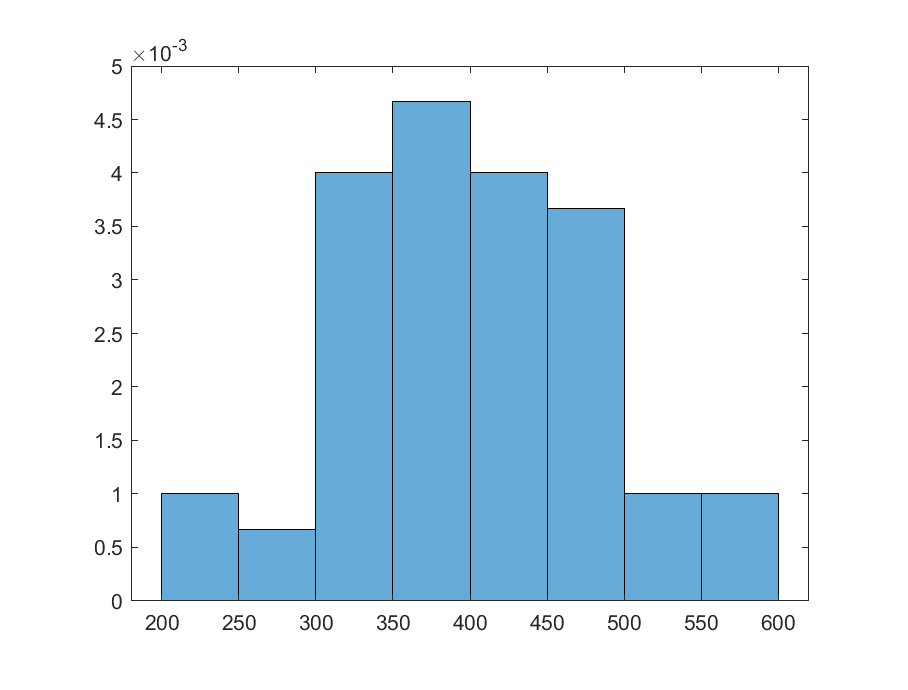
\includegraphics[width = 0.5\textwidth]{images/histogram.eps}

就得到了需要的频率分布直方图.从直方图可以更直观地看到图书馆每日借出图书册数的分布情况.
\end{frame}

\begin{frame}{用样本估计总体分布}
\alert{C、频率折线图}

用$d_1,d_2,\dots,d_k$分别表示频率分布直方图中各矩形上边的中点,在直方图的左边延长出一个分段,分段的中点用$d_0$表示.在直方图的右边也延长出一个分段,分段的中点用$d_{k+1}$表示.

用直线连接$d_0,d_1,\dots,d_{k+1}$就得到了一条折线,这条折线叫做频率折线图.频率折线图也反映出数据频率分布的规律.

下图是例子3.1中图书馆借出图书数据的频率折线图.
\centering
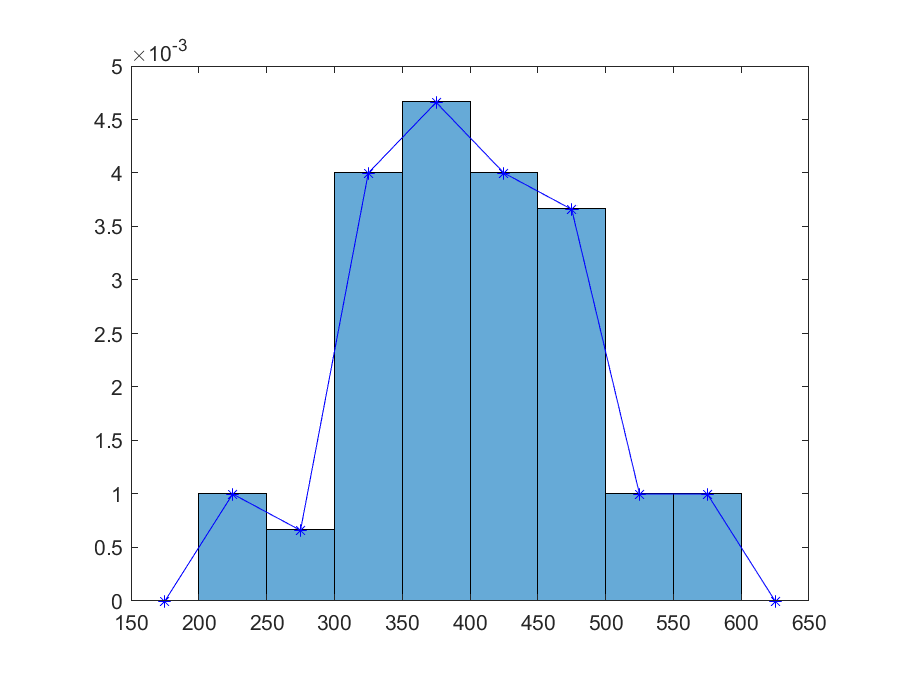
\includegraphics[width = 0.5\textwidth]{images/zhexian.eps}
\end{frame}

	\begin{frame}{用样本估计总体分布}
		\alert{D、数据茎叶图}
		
		直方图主要用于展示分段数据的频率分布,对于没有分段的观测数据还可以用数据的茎叶图展示它的特性.
		
		数据的\alert{茎叶图}由"茎"和"叶"两部分组成,在制作茎叶图的时候要先确定数据的"茎"和"叶".从数据的茎叶图可以看出数据的分布形状以及数据是否对称,是否集中等分布特性.我们通过举例说明茎叶图的制作方法.
		
		例:下面是上海市2004年7月10-31日空气中可吸入颗粒物的监测数据,以这批数据制作茎叶图
		
		85 85 66 71 62 52 55 59 52 62 59 
		70 80 96 97 94 62 51 57 67 96 93
	\end{frame}

	\begin{frame}{用样本估计总体分布}
	解:先将数据从小到大排列得到
	
	51 52 52 55 57 59 59 62 62 62 66 
	67 70 71 80 85 85 93 94 96 96 97\\
	数据的十位上的数是5,6,7,8,9,把他们叫做"茎",排列在下表的第一列,\\
	茎5后面的个位数分别是1,2,2,5,7,9,9,把它们叫做茎5的"叶",排在茎5的后面;\\
	按相同的方法把茎6的叶2,2,2,6,7排在茎6的右边;\\
	$\cdots\cdots\cdots\cdots$\\
	把茎9的叶3,4,6,6,7排在茎9的右边.\\
	就得到了如下的茎叶图
	\end{frame}

	\begin{frame}{用样本估计总体分布}
		$\quad\quad\quad\quad\quad\quad\quad\quad\quad\quad\quad\quad$\begin{tabular}{r|l}
			\hline 茎 & 叶\\
			\hline 5 & 1225799 \\
			\hline 6 & 22267\\
			\hline 7 & 01\\
			\hline 8 & 055\\
			\hline 9 & 34667\\
			\hline
		\end{tabular}
		
		从茎叶图中看出,尽管这22天中可吸入颗粒物都是处于良的水平,但是有较多的时间接近于优,也有较多的时间接近于轻度污染.
		
		数据茎叶图的优点是利用了数据的每个信息,从茎叶图中可以直观地看到数据的分布情况.但是数据量很大时,茎叶图的效果就不好了,因为这是的茎叶图会很长很粗.
	\end{frame}
	
	\begin{frame}{众数和中位数}
		数据的频率分布表、频率分布直方图和茎叶图都可以展示出数据的分布形状,从中可以对数据有一个大致的了解.为了更好地掌握数据的特性和规律,还需要进一步考虑代表数据特征的其他指标.
		\\ \hspace*{\fill} \\
		\alert{A、众数}
		\\ \hspace*{\fill} \\
		我们称观测数据中出现次数最多的数是\alert{众数}(mode),用$M_0$表示.
		
		按照这个定义,在抽样调查中,样本中出现次数最多的数据是样本的众数.
		
		$\quad$如果观测数据中每个数出现的次数都相同,它就没有众数.如果观测数据中有两个或两个以上的数出现次数相同,且出现次数超过其它数的出现次数,这几个数都是众数.
		
		$\quad$众数是观测数据的代表值,它受数据中极大或极小值的影响较小.从分布的角度看,众数出现的频率最高.			
	\end{frame}

	\begin{frame}{(样本)众数和(样本)中位数}
		例子: 某超市用随机抽样的方式调查了30个顾客购买商品的件数,结果从小到大排列如下:
		0,0,1,1,1,2,2,2,3,3,4,5,6,6,8,9,9,10,10,10,10,12,12,13,15,16,18,20,23,29.
		
		求众数和样本均值.
		
		解: 样本中10出现的次数最多,是4次,所以10是众数.样本均值是
		\begin{equation}
			\overline{x} = \frac{1+1+\cdots+23+29}{30} = 8.667.
		\end{equation}
		在此例中,如果购买件数最多的那个顾客购买件数从29增加到40,众数不变,样本均值增加到9.03.
		
		从这个例子中,数据中最大值的变化对众数没有影响,对样本均值的影响较大.
		
		在统计学上,我们将数据的最大值和最小值统一称为极值.称最大值和最小值之差为\alert{极差},$\text{极差} = \text{最大值} - \text{最小值}.$
		
		上例中的极差为$29-0 = 29$,说明所有数据的变化范围或波动幅度不超过29.
	\end{frame}

	\begin{frame}{(样本)众数和(样本)中位数}
		\alert{B、中位数}
		\\ \hspace*{\fill} \\
		设观测数据已经从小到大排列为$x_1\leqslant x_2\leqslant\cdots\leqslant x_n$.
		(1)如果样本量$n$是奇数,我们称中间的数据是\alert{中位数}(median),记作$M_d$.
		\begin{equation}
			M_d = x_m,\text{其中}m = \frac{n+1}{2}.
		\end{equation}
		例如样本1,5,9,12,13的中位数是9.样本4,26,45,67,96,98,112的中位数是67.
		
		(2)如果样本量$n$是偶数,我们称两个中间数据的平均值是中位数,也记作$M_d$.
		\begin{equation}
			M_d = \frac{x_m+x_{m+1}}{2},\text{其中}m = \frac{n}{2}.
		\end{equation}
		例如34,36,45,67,96,98,112,134的中位数是$M_d = (67+96)/2 = 81.5$
	\end{frame}

	\begin{frame}
		由于中位数位于顺序数据的中间,所以有以下性质:
		
		\alert{小于等于中位数的数据不少于样本量的二分之一,大于等于中位数的数据不少于样本量的二分之一}.
		\\ \hspace*{\fill} \\
		例: 2018年,在对A城市工作的某大班同学进行年人均收入(单位:万元)调查时,采用随机抽样的方法得到了以下10个数据:
		
		7.9,9.8,11.7,14.6,16.7,17.9,18.2,19.8,22.6,97.8.
		
		计算中位数和样本均值.
		
		解:数据已经从小到大排列.中位数是$M_d = (16.7+17.9)/2 = 17.3.$
		
		样本均值$\overline{x} = (7.9+9.8+\cdots+97.8) = 23.7.$
		
		在本例中,因为97.8万元的年收入比其他人的年收入高得太多了,所以97.8拉高了样本均值.但是,即使将97.8改为27.8,中位数也不变化.
	\end{frame}

	\begin{frame}{随机对照实验}
		近年来,不断发生的公共安全事故已经成为公众关心的热点.在大洋的彼岸,美国食品药品监督管理局(简称FDA)一直恪守成规,遵照美国的食品和药品法规行事,最大程度地将食品药品安全事故降到最低.尽管如此,在20世纪80年代上市的抗心律失常药Tambocor(氟卡胺)和Enkaid(英卡胺)等还是引发了一次重大药害事件.短短的几年内,估计有5万人因服用这类药物导致心脏骤停而死亡.下面的内容选自[Thomas J. Moore. 《致命的药物》]
	\end{frame}

	\begin{frame}{随机对照实验}
		在20世纪80年代,3M是美国最大的公司之一,曾在财富500强中名列第47位。它因买下一个小型制药公司,再经过10多年的研发,终于有了自己的新药Tambocor(氟卡胺)。新药的上市,成了3M公司的摇钱树。13年来,Tambocor曾在小鼠、大鼠、兔子、猪、狗、猫和狒狒体内进行了试验研究。1975年,FDA批准了Tambocor的临床研究申请,1975-1978年,对于Tambocor的I期和II期临床试验结果比较令人满意。与此同时,百时美公司也加快了同类药品Enkaid(英卡胺)的研发速度。
		
		20世纪70年代,用药物预防心率失常的理论开始流行,尽管缺乏充分的科学依据,1979年医生开出了1200万次处方药,这些事实强烈刺激着3M的Tambocor研发。
		
	\end{frame}

	\begin{frame}{随机对照实验}
		1982年,德国批准了Tambocor的销售。接下来,斯坦福大学的温克医生发表文章讲述了Enkaid导致了一些重症患者的死亡。Tambocor和Enkaid的化学结构相似,但是不一定又相同的问题。温克医生和3M公司讨论Tambocor时,提出在重症患者中试验Tambocor,而3M公司只想在有室性早搏症,且身体健康的人群中试验Tambocor。
		
		1982年11月,3M公司邀请了医学界的专家分析临床试验数据。在45家医院服用Tambocor的患者中,Tambocor没有表现出良好的疗效,反而导致了部分患者的死亡。Enkaid也遇到 了同样的问题。\alert{可惜的是,因为没有统一的试验方案,研究人员很难对于这些数据加以统计分析。}尽管如此,在进一步的试验结果出来之前,3M公司还是按原计划向FDA提交了新药上市的申请。
	\end{frame}

	\begin{frame}{随机对照实验}
		1983年,3M公司在旅游圣地百慕大召开了Tambocor的研讨会,3M支付了全部费用,除了温克医生继续表示担忧外,大部分收了报酬的专家对Tambocor给予热情的支持。
		
		1985年10月8日,在缺乏严密的试验数据的情况下,Tambocor及其同类药物获得上市批准。新一代抗心律失常药开始大量涌向市场。之后,3M借助推销、广告、研讨会等大力推广Tambocor。1988年春,美国的医生每月平均开出57000张Tambocor处方。
		
		1986年12月,FDA批准了Enkaid上市。在一个以市场促销为目的的临床试验中,6周内Enkaid导致了39人死亡。至此,FDA、制药公司和医生都注意到这类药会导致心脏骤停,但是他们认为这些药利大于弊。百时美和3M公司继续开动着赚钱机器。
	\end{frame}

	\begin{frame}{随机对照实验}
		幸运的是,在抗心律失常药被审批和销售的同时,美国心肺血液研究所开始对这类药物进行大规模的心律失常抑制试验(简称CAS试验)。试验包括Tambocor和Enkaid等,涉及4400位患者,27个研究中心和100多家医院,耗时5年,耗资4400万美元。
		
		CAS试验严格按照\alert{随机对照双盲试验}的原则进行:把每个患者随机地分在X组或Y组,为其中一组提供药品,为另一组提供\alert{安慰剂}(貌似药物,但无任何药效)。这是随机对照的含义。不管是研究人员还是患者,除了生物统计学家霍尔斯乔姆一人,没人知道哪些是真药,哪些是安慰剂。这是双盲的含义。谁也没有权利过问治疗组(服用真药的组)和对照组(服用安慰剂的组)的身份情况,由于霍尔斯乔姆默默地保守着秘密,使得想为药品讲话的医生也无从开口,大家只能默默地等待试验的进展。
	\end{frame}	

	\begin{frame}{随机对照实验}
		到1988年9月1日,CAS试验的内部结果如下(其中的猝死人数包括心脏骤停但是抢救成功的患者)。
		
		$\quad\quad\quad\quad\quad\quad\quad\quad\quad$\begin{tabular}{l|l|l}
			\hline  & X组 & Y组\\
			\hline 患者总数 & 576 & 571\\
			\hline 猝死人数 & 3 & 19 \\
			\hline
		\end{tabular}
		
		可以看出,Y组的猝死率是X组的6.38倍。这样的差异大大超出了随机因素所能解释的范围。事实上,对该数据进行如下的假设检验,设原假设H0: 该药物与猝死无关 vs 备择假设H1: 该药物与猝死有关,由调查数据得到:
		
		$\quad\quad\quad\quad\quad\quad\quad$\begin{tabular}{l|l|l}
			\hline 统计量 & 值 & P值 \\
			\hline 卡方 & 12.0068 & 0.0005\\
			\hline 似然比卡方检验 & 13.3432 & 0.0003 \\
			\hline 连续调整卡方 & 10.5612 & 0.0012 \\
			\hline Mantel-Haenszel 卡方 & 11.9963 & 0.0005 \\
			\hline
		\end{tabular}
	\end{frame}	

	\begin{frame}{随机对照实验}
		可以看到,无论是上述的哪一种检验方法,其P值都远小于0.01,所以这个检验是高度显著的,我们可以肯定地说,根据CAS试验,认为该药物与猝死有关时,所犯错误的概率不会超过α=0.01,我们应当否认该药物与猝死无关。随着试验的继续,两组间的差异没有缩小,趋势也没有发生转变。因为患者是被随机分配到X组和Y组的,所以结论表明,不是该药品有效,就是该药品致命。
		
		现在,我们已经知道了,X组是安慰剂组,Y组是试验组。随机对照双盲试验清楚地揭示了Tambocor和Enkaid的确是致命的药物。CAS试验中止后,CAS试验项目长官弗里德曼在给3M公司的信中写道:“采取这个行为是因为Tambocor经证明基本不可能存在疗效,反而它很可能对该患者群体有危害”。
		
	\end{frame}

	\begin{frame}{随机对照实验}
		在CAS试验中,称使用真药的人在试验组,使用安慰剂的人在对照组。通常,实验组由随机选择出的对象构成,试验组的成员接受特殊的待遇或治疗。而对照组由那些没有接受过这种特殊待遇的对象构成,通常为他们提供的是安慰剂。任何好的试验设计应当有一个实验组和对照组。
		
		在CAS试验中,如果没有对照组,为所有的患者提供药品,就无法确认Tambocor和Enkaid会造成心脏骤停的结论。如果试验组和对照组不是随机选择的,由于两组人群的差异,也无法分析出正确的结论。同样,不让医生和患者知道患者在哪一组,甚至不让他们知道安慰剂的存在,是为了得到没有偏见的数据。
	\end{frame}	

	\begin{frame}{随机对照实验}
		当然,随机对照试验也会遇到道德方面的谴责。在决定停止对Tambocor和Enkaid的CAS试验时,就有医生愤怒指责CAS试验“不道德”。因为一旦试验证明药品有效,那么分在对照组的一半人就没有得到治疗。有这样想法的医生并不少。因为当时有一半的医生在治疗心脏早搏,都以为自己在帮助患者。但是,CAS试验的结论证明,他们正在无意中杀害自己的患者。
		
		Rmk:上述抗心律失常药对于部分轻度心律失常患者有效.
		
		随机选择试验对象是英国统计学家Fisher的贡献,在20世纪初,他用此方法致力于农业试验对象的研究。从此,随机选择试验组成为安排试验的基本原则。下面的例子来自[Freedman D.《统计学》]、[Iverson G R, Gergen M.《统计学》]、[Grace N D,et al. The present status of shunts for protal hypertension in cirrhosis. Journal of Gastroenterology.1966,50,686-691]、[Sacks H, Chalmer T C and Smith H. Randomized versus historical controls for clinical trials. American Journal of Medicine,1982,72,233-240]
		
	\end{frame}	
	
	\begin{frame}{随机对照实验}
		例(静脉吻合分流术)在一些肝硬化病例中,许多患者会从肝出血直至死亡.历史上有一种称为"静脉吻合分流术"的外科手术用于治疗肝硬化,其原理是用外科手术的方法使血流改变方向.这种手术花费很大并且有很高的危险性.值得做这样的手术吗?
		
		为了解决上述问题,一共有三批共51次手术试验.第一批进行了32次无对照组的试验.结果如下:
		
		$\quad\quad\quad\quad$\begin{tabular}{|c|c|c|c|c|}
			\hline 设计方法 & 试验次数 & 显著有效 & 中等有效 & 无效\\
			\hline 无对照组 & 32 & 24 & 7 & 1\\
			\hline 所占比例 &    & 75\% & 21.9\% & 3.1\% \\
			\hline
		\end{tabular}
	
		试验说明75\%的手术显著有效,21.9\%的手术中等有效,看来手术是值得做的.
	\end{frame}
	
	\begin{frame}{随机对照实验}
		第二批共进行了15\%次手术试验,这批试验有对照组,但是对照组的患者不是随机选取的.医生根据患者的临床诊断情况决定是将患者编入试验组做手术,还是编入对照组不做手术.结果如下:
		
		$\quad\quad\quad\quad$\begin{tabular}{|c|c|c|c|c|}
			\hline 设计方法 & 试验次数 & 显著有效 & 中等有效 & 无效\\
			\hline 非随机对照 & 15 & 10 & 3 & 2\\
			\hline 所占比例 &    & 66.7\% & 20\% & 13.3\% \\
			\hline
		\end{tabular}
	
		这次试验的结果是66.7\%的手术显著有效,20\%的手术中等有效,13.3\%的手术无效.这个试验结果也是对"静脉吻合分流术"的肯定.这次的结果与无对照组的试验结果差别不是很大.
	\end{frame}
	
	\begin{frame}{随机对照实验}
		再看有随机选取的对照组的第三批试验,这批试验只有4次手术.随机选取的方式类似于掷硬币,如果硬币正面朝上就将患者选入试验组做手术.这次试验的结果如下:
		
		$\quad\quad\quad\quad$\begin{tabular}{|c|c|c|c|c|}
			\hline 设计方法 & 试验次数 & 显著有效 & 中等有效 & 无效\\
			\hline 随机对照 & 4 & 0 & 1 & 3\\
			\hline 所占比例 &    & 0\% & 25\% & 75\% \\
			\hline
		\end{tabular}
	
		随机对照试验的结果显著地否定了外科手术"静脉吻合分流术"的价值.经过认真设计的试验研究显示"静脉吻合分流术"几乎没有什么价值.
	\end{frame}
	
	\begin{frame}{随机对照实验}
		为什么会出现如此大的差别呢?
		
		在无对照组和非随机选取对照组的试验中,试验者根据患者的临床诊断决定是否将他编入试验组进行手术.这样就做出现一种自然的倾向:试验人员更倾向于将那些身体状态较好的患者选入试验组,以减少手术风险.其结果有利于对手术的肯定评价,这种结果是不真实的.
		
		对上述试验的跟踪观测发现,做手术的51个患者中3年后大约有60\%仍然活着,随机对照组中(没做手术的患者)3年后大约也有60\%仍然活着.这说明手术基本是无效的.而在非随机对照组中,只有45\%的患者存活期超过三年,这说明了非随机对照组中的患者健康情况较差,验证了健康情况较好的患者更容易被选入试验组做手术.
		
		随机安排对照组是十分必要的,否则可能得出错误的结论.我们称随机选取试验组的对照试验为\alert{随机对照试验}.在随机对照试验中,为了得到更真实的结果,有时还需要其他的手段配合.
	\end{frame}		
	\begin{frame}{随机对照实验}
		在人类历史上,还有许多成功使用随机对照试验的例子,也有许多惨痛的教训。例如,随机对照试验否定了治疗冠状动脉病的冠状动脉旁道外科手术(该手术费用昂贵),否定了用抗凝剂治疗心脏病突发,否定了用5-FU对结肠癌进行化疗,否定了用己烯雌酚预防流产.具体情况如下:
		\\ \hspace*{\fill} \\%空行
		$\quad\quad\quad$\begin{tabular}{|c|c|c|c|c|}
			\hline 医疗方法 & \multicolumn{2}{|c|}{随机对照试验} & \multicolumn{2}{|c|}{非随机对照试验}\\
			\hline 结论 & 有效 & 无效 & 有效 & 无效 \\
			\hline 冠状旁道外科手术 & 1 & 7 & 16 & 5 \\
			\hline 抗凝剂治疗 & 1 & 9 & 5 & 1 \\
			\hline 5-FU结肠癌化疗 & 0 & 5 & 2 & 0 \\
			\hline 己烯雌酚预防流产 & 0 & 3 & 5 & 0 \\
			\hline
		\end{tabular}
		
	\end{frame}	
		
	\begin{frame}{随机对照实验}	
		特别需要指出的是有关己烯雌酚的试验,随机对照试验完全否定了这种预防流产的药物。而历史上糟糕的非随机对照试验缺赞同药物的疗效,这是一个医学的悲剧。在20世纪60年代末的美国,医生每年大约为5万名孕妇发放这种药。后来揭示,怀孕期间的母亲服用己烯雌酚,20年后将给她们的女儿带来灾害性的副作用,可能引发她们的女儿得一种罕见的癌症。该药于1971年被禁止使用。
		
		人们从太多的悲剧中总结了教训:对一种新药不作随机对照试验是非常危险的。
			
	\end{frame}	
	
	\begin{frame}
		例: 1916年小儿麻痹症(脊髓灰质炎)袭击了美国,以后的40年间,受害者成千上万.20世纪50年代,人们开始发现预防疫苗.当时萨凯(Salk)培育的疫苗最有希望.他的疫苗在试验室表现良好:安全,产生对脊髓灰质炎病毒的抗体.但是在大规模使用前必须进行现场人体试验,通过试验最后确定疫苗是否有效.只有这样才能达到保护儿童的目的.
		
		当时采用了随机对照的研究方案,对每个儿童用类似投掷一个硬币的方法决定是否将他编入试验组:正面朝上分在试验组,否则分在对照组.除了试验的设计人员,连医生也不知道哪个儿童分在试验组,哪个儿童分在对照组.
		
		然后给分在试验组的儿童注射疫苗,给分在对照组的儿童注射生理盐水,让他们认为也被注射了疫苗.得到的结果如下:
		
		$\quad\quad\quad\quad$\begin{tabular}{|c|c|c|}
			\hline & 试验人数 & 试验后的发病率 \\
			\hline 试验组 & 20万 & 28/10万 \\
			\hline 对照组 & 20万 & 71/10万 \\
			\hline
		\end{tabular}
	
		试验结果显示,疫苗将小儿麻痹症的发病率从10万分之71降低到10万分之28.由于71和28的差别超出了随机性本身所能解释的范围,所以宣布疫苗是成功的.进一步的分析指出,可以以近100\%的概率保证疫苗是有效的(见后面的显著性检验一节).
	\end{frame}
	
	\begin{frame}{随机对照实验}
		上例中的安慰剂是注射生理盐水,给对照组的儿童使用安慰剂是为了避免儿童的心理作用影响试验的结果.尽管可以认为仅靠精神作用不能抵抗小儿麻痹症,但是为了确认试验结果的可靠性,使用安慰剂是必要的.
		
		上例中的随机对照试验是双盲的.双盲的之一是指儿童自己不知道自己是在试验组还是在对照组,也就是说不知道自己被注射的是疫苗还是生理盐水(安慰剂),甚至不知道有安慰剂,这就有效地避免了潜在的心理影响.另外一盲是指医生不了解他诊断的患者是在对照组还是在试验组,这就避免了医生对疫苗的主观看法带来的可能影响.在可能的场合,随机对照双盲试验可以最大程度地避免心理因素的影响.
		
		在许多场合,心理因素是不能忽视的.有资料显示在医院中给那些手术后产生剧痛的患者服用用淀粉制成的"止痛片"后,大约有1/3的患者感觉剧痛减轻.		
	\end{frame}

	\begin{frame}
		练习:用$s_x^2$表示$x_1,\dots,x_n$的样本方差,用$b$表示常数,用$s_y^2$表示$y_1,\dots,y_n$的样本方差.当$y_1=x_1+b,y_2=x_2+b,\dots,y_n=x_n+b$时,验证$s_y^2 = s_x^2$.
		\\ \hspace*{\fill} \\%空行
		练习:某学苑超市销售部收到甲乙两厂送来的质地相同的可乐各10瓶,测量后得到甲乙两厂可乐的净含量(单位:ml)分别是:
		$\quad\quad\quad\quad$\begin{tabular}{|c|c|c|c|c|c|c|c|c|c|c|}
			\hline 甲厂 & 501 & 500 & 499 & 500 & 502 & 500 & 500 & 501 & 499 & 498 \\
			\hline 乙厂 & 497 & 501 & 500 & 502 & 499 & 501 & 503 & 500 & 500 & 497 \\
			\hline
		\end{tabular}
	
		问:销售部应当销售哪家的冰可乐.
		\\ \hspace*{\fill} \\%空行
		练习:用自己的话叙述什么是对照组、什么是试验组、什么是随机对照试验.
	\end{frame}
\section{参数的估计方法}
 \frame{\sectionpage}

	\begin{frame}{样本均值和样本方差}
		如果$X$是从总体中随机抽出的个体,则$X$是随机变量,$X$的分布就是总体的分布.如果对总体进行有放回的抽样,则得到独立同分布且和$X$同分布的随机变量$X_1,X_2,\cdots,X_n$.这时称$X_1,X_2,\cdots,X_n$是来自总体$X$的\alert{简单随机样本},简称为总体$X$的\alert{样本}.
		
		$\quad$在观测放射性钋(pō)放射$\alpha$粒子的试验中,用$X$表示7.5s内观测到的粒子数.独立重复观测时,用$X_i$表示第$i$次的观测结果,则$X_1,X_2,\cdots,X_n$独立同分布且和$X$同分布,$X_1,X_2,\cdots,X_n$是总体$X$的样本.
		
		Def1.1 如果$X_1,X_2,\cdots,X_n$独立同分布且和$X$同分布,则称$X$是总体,称$X_1,X_2,\cdots,X_n$是总体$X$的样本,称观测数据的个数$n$为样本量.
	\end{frame}

	\begin{frame}{样本均值和样本方差}
		在实际问题中得到的总是简单随机样本$X_1,X_2,\cdots,X_n$的观测值$x_1,x_2,\cdots,x_n$,人们也称$x_1,x_2,\cdots,x_n$是总体$X$的样本.在统计学中,常常不把$X_1,X_2,\cdots,X_n$与它们的观测值$x_1,x_2,\cdots,x_n$严格区分,这是为了符号使用的方便.当对数据进行统计分析时,用大写的$X_1,X_2,\cdots,X_n$,实际计算时更多地用小写的$x_1,x_2,\cdots,x_n$.
		\\ \hspace*{\fill} \\%空行
		在统计问题中,总体$X$的分布形式往往是已知的.例如重复测量一个物体的重量时,认为总体$X$服从正态分布$N(\mu,\sigma^2)$,未知参数是$\mu,\sigma^2$,问题是根据总体$X$的样本估计总体参数$\mu,\sigma^2$. 观测放射物钋放射$\alpha$粒子时,总体$X$服从泊松分布$\mathcal{P}(\lambda)$,未知参数是$\lambda$,问题是根据总体$X$估计参数$\lambda$.
	\end{frame}

\section{抽样分布}
 \frame{\sectionpage}
	\begin{frame}{抽样分布}
		$\chi^2$分布、$t$分布、$F$分布是统计学中最重要的抽样分布,被称为统计学中的三大分布.本节的任务是推导这三个分布.
		
		抽样分布是统计推断的基础,其理论证明是概率统计课中不可绕过的一个难点.
		
		(1)$\chi^2$分布
		
		设$X_1,...,X_n$是总体$X\sim N(0,1)$的样本,则\alert{平方和
		\begin{equation}
			\xi_n^2 = X_1^2+...+X_n^2
		\end{equation}
		服从$n$个自由度的$\chi^2$分布},有概率密度
		\begin{equation}
			f_n(z) = \frac{1}{2^{n/2}\Gamma(n/2)}z^{n/2-1}e^{-z/2}\bm{1}_{(z>0)}
		\end{equation}
		记作: $\xi_n^2\sim \chi^2(n)$
	\end{frame}

	\begin{frame}
		证明: 往证$Y_k = X_k^2\sim \Gamma(\frac{1}{2},\frac{1}{2})$.
		
		注意到: $\{Y_k = y\} = \{X_k = \sqrt{y}\}\cup\{X_k = -\sqrt{y}\}$,

		故$Y_k$的密度函数是:
		\begin{equation}
			\begin{split}
				f_{Y_k}(y) &= \varphi(\sqrt{y})\frac{1}{2\sqrt{y}} + \varphi(-\sqrt{y})\frac{1}{2\sqrt{y}}\\
				&= \frac{1}{\sqrt{2\pi y}}e^{-y/2}\bm{1}_{(y>0)}.
			\end{split}
		\end{equation}
		这正是$\Gamma(\frac{1}{2},\frac{1}{2})$的概率密度函数,故$Y_k = X_k^2\sim \Gamma(\frac{1}{2},\frac{1}{2})$.
		
		再由$\Gamma$分布的可加性知道:
		\begin{equation}
			\xi_n^2 \sim \Gamma(\frac{n}{2},\frac{1}{2})
		\end{equation}
		因此,它有概率密度函数$f_n(z) = \frac{1}{2^{n/2}\Gamma(n/2)}z^{n/2-1}e^{-z/2}\bm{1}_{(z>0)}$
	\end{frame}

	\begin{frame}	
		另解: 先求分布函数,之后对分布函数求导得概率密度.
		
		$Y_k$有分布函数
		\begin{equation}
		\begin{split}
			F_{Y_k}(y) &= P(X_k^2\leqslant y)  = P(-\sqrt{y}\leqslant X_k\leqslant \sqrt{y}) \\
			&= \varPhi(\sqrt{y}) - \varPhi(-\sqrt{y}) = 2\varPhi(\sqrt{y}) - 1.
		\end{split}
		\end{equation}
		
		因此,
		\begin{equation}
		\begin{split}
			f_{Y_k}(y) &= F_{Y_k}'(y) \\
			&= 2\times\frac{1}{2\sqrt{y}}\varphi(\sqrt{y}) \\
			&= \frac{1}{\sqrt{2\pi y}}e^{-y/2}\bm{1}_{(y>0)}.
		\end{split}
		\end{equation}
		下同第一种解法.
	\end{frame}


	\begin{frame}{$\chi^2$分布}
		\centering
		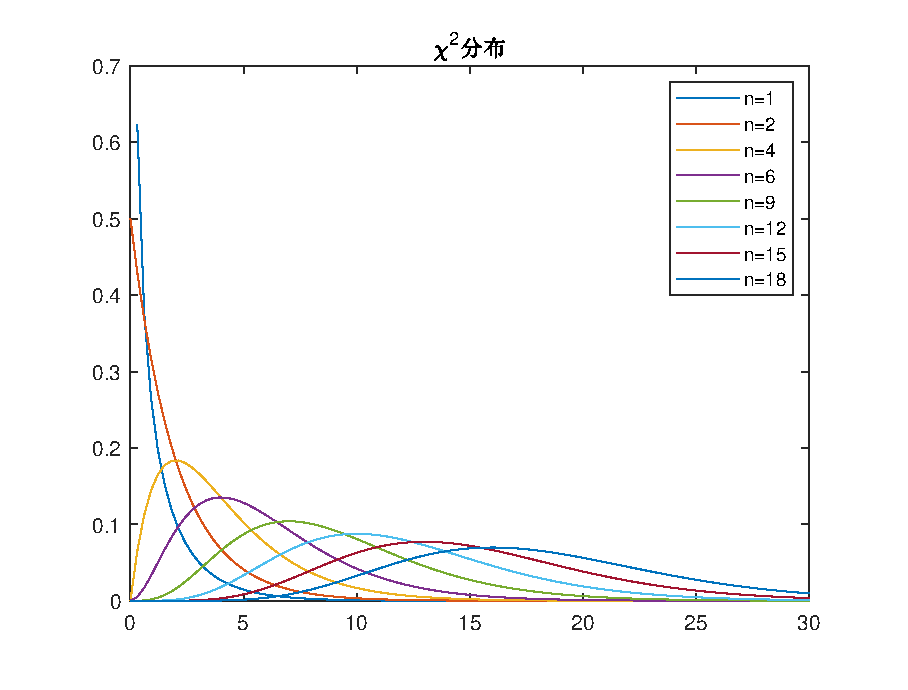
\includegraphics[width = 0.9\textwidth]{images/chi2.eps}
	\end{frame}

	\begin{frame}
		(2)$t$分布
		
		设随机变量$X\sim N(0,1),Y\sim \chi^2(n)$,其中$X,Y$独立,则\alert{随机变量
		\begin{equation}
			T = \frac{X}{\sqrt{Y/n}}
		\end{equation}
		服从n个自由度的$t$分布},并且有概率密度
		\begin{equation}
			f_T(t) = a_n \bigg(1+\frac{t^2}{n}\bigg)^{-\frac{n+1}{2}},
		\end{equation}
		其中$a_n = \frac{1}{\sqrt{n}\mathrm{B}(n/2,1/2)}$是归一化的系数.
	\end{frame}
	
	\begin{frame}{$t$分布}
		证明:(法一)增补变量$S = Y$,来求$(T,S)$的联合概率密度函数$g(t,s)$.
		
		$(X,Y)$有联合密度函数$f(x,y) = \frac{1}{\sqrt{2\pi}}e^{-x^2/2} \frac{1}{2^{n/2}\Gamma(n/2)}y^{n/2-1}e^{-y/2}\bm{1}_{(y>0)}$
		
		注意到: $\{(T,S)=(t,s)\} = \{(X,Y) = (t\sqrt{s/n},s)\}$,
		
		Jacobi阵为:$J = \begin{pmatrix} \sqrt{s/n} & * \\ 0 & 1 \end{pmatrix}$,$|\det(J)| = \sqrt{s/n}$,故有:
		\begin{equation}
			\begin{split}
				g(t,s) &= f(t\sqrt{s/n},s) \sqrt{s/n} \\
				&= \frac{1}{\sqrt{2\pi}}e^{-\frac{t^2s}{2n}} \frac{1}{2^{n/2}\Gamma(n/2)}s^{n/2-1}e^{-s/2}\bm{1}_{(s>0)}\sqrt{s/n} \\
				&= c_n s^{\frac{n-1}{2}}\exp(-\frac{1}{2}(\frac{t^2}{n}+1)s)\bm{1}_{(s>0)}
			\end{split}
		\end{equation}
		因此,$T$的概率密度为$f_T(t) = \int_{0}^{\infty}g(t,s)\mathrm{d}s$
	\end{frame}
	
	\begin{frame}
		为计算该式,替换$u = \frac{1}{2}(\frac{t^2}{n}+1)s$,便有:
		\begin{equation}
			\begin{split}
				f_T(t) &= \int_{0}^{\infty}g(t,s)\mathrm{d}s \\
				&= c_n\int_{0}^{\infty}s^{\frac{n-1}{2}}\exp(-\frac{1}{2}(\frac{t^2}{n}+1)s)\mathrm{d}s \\
				&= 2^{\frac{n-1}2}c_n\bigg[\int_{0}^{\infty}u^{\frac{n-1}{2}}\exp(-u)\mathrm{d}s\bigg] \bigg(1+\frac{t^2}{n}\bigg)^{-\frac{n+1}{2}} \\
				&= a_n \bigg(1+\frac{t^2}{n}\bigg)^{-\frac{n+1}{2}}.
			\end{split}
		\end{equation}
		其中$a_n = 2^{\frac{n-1}2}c_n \Gamma(\frac{n+1}{2}) = \frac{1}{\sqrt{2\pi}}\frac{2^{\frac{n-1}2}}{2^{n/2}\Gamma(n/2)}\frac{1}{\sqrt{n}}\Gamma(\frac{n+1}{2}) = \frac{1}{\sqrt{n}\mathrm{B}(n/2,1/2)}$.
	\end{frame}

	\begin{frame}
		$a_n$的计算也可以由$\int_{-\infty}^{\infty}f_T(t)=1$得到:
		
		\begin{equation}
			\begin{split}
			\frac{1}{a_n} &= 2\int_{0}^{\infty}\bigg(1+\frac{t^2}{n}\bigg)^{-\frac{n+1}{2}}\mathrm{d}t \\
			&= \sqrt{n}\int_{0}^{1}s^{n/2-1}(1-s)^{1/2-1}\mathrm{d}s \big[\text{取变换}1+\frac{t^2}{n}=\frac{1}{s}\big] \\
			&= \sqrt{n}\mathrm{B}(n/2,1/2)
			\end{split}
		\end{equation}
	\end{frame}

	\begin{frame}
		证明:(法二) 先求概率分布,再求导得概率密度.
		
		$(X,Y)$有联合密度函数$f(x,y) = \frac{1}{\sqrt{2\pi}}e^{-x^2/2} \frac{1}{2^{n/2}\Gamma(n/2)}y^{n/2-1}e^{-y/2}\bm{1}_{(y>0)}$
		
		
		\begin{equation}
			\begin{split}
				F_T(t) &= P(T\leqslant t) = \iint\limits_{\{x\leqslant t\sqrt{y/n}\}}f(x,y)\mathrm{d}x\mathrm{d}y \\
				&= \int_{0}^{\infty}\varPhi(t\sqrt{y/n})\frac{1}{2^{n/2}\Gamma(n/2)}y^{n/2-1}e^{-y/2} \mathrm{d}y
			\end{split}
		\end{equation}
		对上式求导得到:
		\begin{equation}
			\begin{split}
				f_T(t) &= F_T'(t) \\
				&= \int_{0}^{\infty}\varphi(t\sqrt{y/n})\sqrt{y/n}\frac{1}{2^{n/2}\Gamma(n/2)}y^{n/2-1}e^{-y/2} \mathrm{d}y \\
				&=\frac{1}{\sqrt{2\pi n}2^{n/2}} \int_{0}^{\infty} y^{\frac{n-1}{2}}\exp(-\frac{1}{2}(\frac{t^2}{n}+1)y) \mathrm{d}y \quad\text{下同法一}
			\end{split}
		\end{equation}
	\end{frame}



	\begin{frame}{$t$分布}
		\centering
		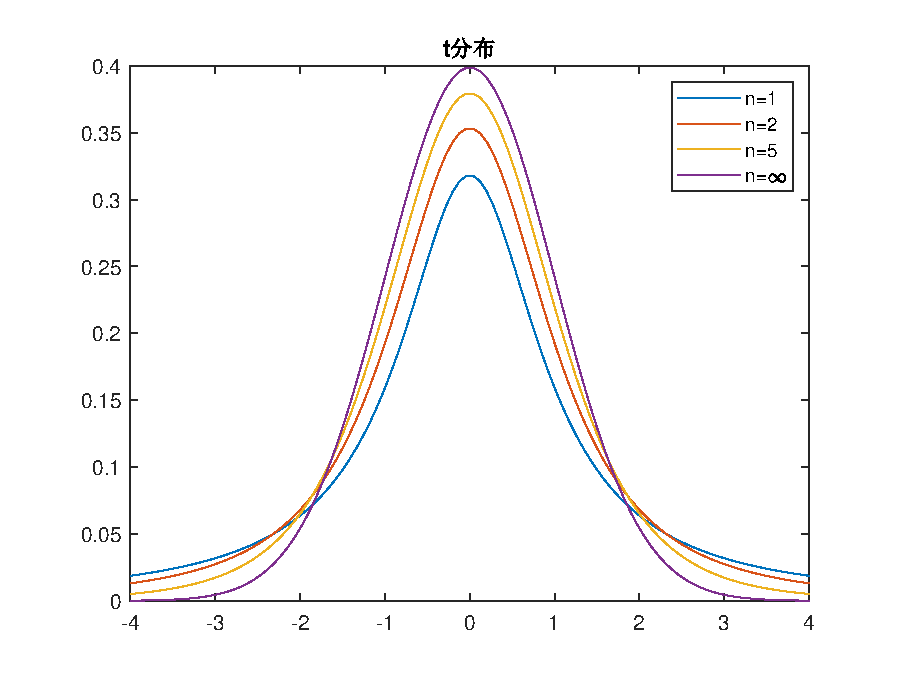
\includegraphics[width = 0.9\textwidth]{images/student(t).eps}
	\end{frame}

	\begin{frame}{$F$分布,注意:分子的自由度在前}
		设$X,Y$独立,分别服从自由度是$n,m$的$\chi^2$分布,则
		\alert{
		\begin{equation}
			Z = \frac{X/n}{Y/m}
		\end{equation}
		服从自由度为$n,m$的$F$分布},有概率密度
		\begin{equation}
			f_Z(z) = cz^{n/2-1}\bigg(1+\frac{nz}{m}\bigg)^{-(n+m)/2}\bm{1}_{(z>0)}.
		\end{equation}
		其中,归一化常数$c = (n/m)^{n/2}[\mathrm{B}(n/2,m/2)]^{-1}$.
	\end{frame}

	\begin{frame}{$F$分布,注意:分子的自由度在前}
		证明:(法一)先求概率分布,再求导得概率密度.
		
		由于$Z = \frac{m}{n}\frac{X}{Y}$,故先计算$U =\frac{X}{Y}$的密度$f_U(u)$,
		
		自然得到$Z$的密度$f_Z(z) = \frac{n}{m}f_U(\frac{n}{m}z)$.
		
		$(X,Y)$有联合密度:$f(x,y) = c_1x^{n/2-1}e^{-x/2}y^{m/2-1}e^{-y/2}\bm{1}_{(x>0,y>0)}$
		
		\begin{equation}
			\begin{split}
				F_U(u) &= P(U\leqslant u) = P(X\leqslant uY) \\
				&= c_1\int_{0}^{\infty} \bigg(\int_{0}^{uy}x^{n/2-1}e^{-x/2}y^{m/2-1}e^{-y/2} \mathrm{d}x\bigg)\mathrm{d}y
			\end{split}
		\end{equation}
		求导得:
		\begin{equation}
		\begin{split}
			f_U(u) &=  c_1\int_{0}^{\infty} y(uy)^{n/2-1}e^{-(uy)/2}y^{m/2-1}e^{-y/2} \mathrm{d}y \\
			&= c_1 \int_{0}^{\infty}u^{n/2-1}y^{(n+m)/2-1}\exp (-\frac{1}{2}(1+u)y) \mathrm{d}y
		\end{split}
		\end{equation} 
	
	\end{frame}


	\begin{frame}
		替换$t = \frac{1}{2}(1+u)y$,计算得到:
		\begin{equation}
			\begin{split}
				f_U(u) &= c_2 [\int_{0}^{\infty} t^{(n+m)/2-1}\exp (-t) \mathrm{d}t][\frac{1}{2}(u+1)]^{-(n+m)/2} u^{n/2-1} \\
				&= c_3 [(u+1)]^{-(n+m)/2} u^{n/2-1}, u>0
			\end{split}
		\end{equation}
		于是知道$Z$的密度
		\begin{equation}
			\begin{split}
				f_Z(z) &= \frac{n}{m}f_U(\frac{n}{m}z) \\
				&= c_4 [(\frac{n}{m}z+1)]^{-(n+m)/2} (\frac{n}{m}z)^{n/2-1}, z>0
			\end{split}
		\end{equation}
	\end{frame}

	\begin{frame}
		常数$c_4$的计算可以按照前面的计算过程一步一步计算下来,也可以利用归一化来计算:
		\begin{equation}
			\begin{split}
				\frac{1}{c_4} &= \int_{0}^{\infty}[(\frac{n}{m}z+1)]^{-(n+m)/2} (\frac{n}{m}z)^{n/2-1}\mathrm{d}z \\
				&=\int_{0}^{1} (\frac{1}{s}-1)^{n/2-1}s^{(n+m)/2}\frac{m}{ns^2}\mathrm{d}s,[1+nu/m=\frac{1}{s}] \\
				&=\frac{m}{n}\int_{0}^{1}(1-s)^{n/2-1}s^{m/2-1}\mathrm{d}s \\
				&=\frac{m}{n}\mathrm{B}(n/2,m/2).
			\end{split}
		\end{equation}
	
	\end{frame}

	\begin{frame}
		(法二):增补变量$W = X+Y$,来求$(Z,W)$的联合概率密度函数$g(z,w)$.
		
		事件\begin{equation}
			\begin{split}
				\{Z=z,W=w\} &= \{\frac{m}{n}\frac{X}{Y}=z,X+Y=w \} \\
				 &= \{ X=\frac{\frac{zn}{m}w}{1+\frac{zn}{m}}, Y =\frac{w}{1+\frac{zn}{m}} \}
			\end{split}
		\end{equation}
		\begin{equation}
			\begin{split}
				|\det(J)| &= \bigg| \det\bigg(\frac{\partial(z,w)}{\partial(x,y)}\bigg) \bigg|^{-1} \\
				&=\bigg| \det \begin{pmatrix} \frac{m}{ny} & -\frac{m}{n}\frac{x}{y^2} \\ 1 & 1 \end{pmatrix}\bigg|^{-1} \\
				&= \frac{n}{m}\frac{y^2}{x+y} = \frac{n}{m}\frac{w}{(1+zn/m)^2}.
			\end{split}
		\end{equation}
	\end{frame}

	\begin{frame}
		因此,得到$(Z,W)$的联合概率密度函数
		\begin{equation}
			\begin{split}
				g(z,w) = f(\frac{\frac{zn}{m}w}{1+\frac{zn}{m}},\frac{w}{1+\frac{zn}{m}})\frac{n}{m}\frac{w}{(1+zn/m)^2},
			\end{split}
		\end{equation}
		其中,$f(x,y)$是$(X,Y)$的概率密度函数.
		将上式经过化简,得到:
		\begin{equation}
			g(z,w) = \frac{1}{2^{\frac{m+n}{2}}\Gamma{\big(\frac{m+n}{2}\big)}}w^{\frac{m+n}{2}-1}e^{-\frac{w}{2}}
			\frac{(n/m)^{n/2}}{\mathrm{B}(m/2,n/2)}z^{n/2-1}(1+\frac{zn}{m})^{-(m+n)/2}
		\end{equation}
		巧了!观察上式发现$g(z,w)$可分离变量,且$(Z,W)$的取值区域为矩形区域.
		
		故随机变量$W$和$Z$独立,
			
		$W$有密度$\frac{1}{2^{\frac{m+n}{2}}\Gamma{\big(\frac{m+n}{2}\big)}}w^{\frac{m+n}{2}-1}e^{-\frac{w}{2}}$.
		
		$Z$有密度$\frac{(n/m)^{n/2}}{\mathrm{B}(m/2,n/2)}z^{n/2-1}(1+\frac{zn}{m})^{-(m+n)/2}$,证毕.
		

		
	\end{frame}

	\begin{frame}{$F$分布,注意:分子的自由度在前}
		\centering
		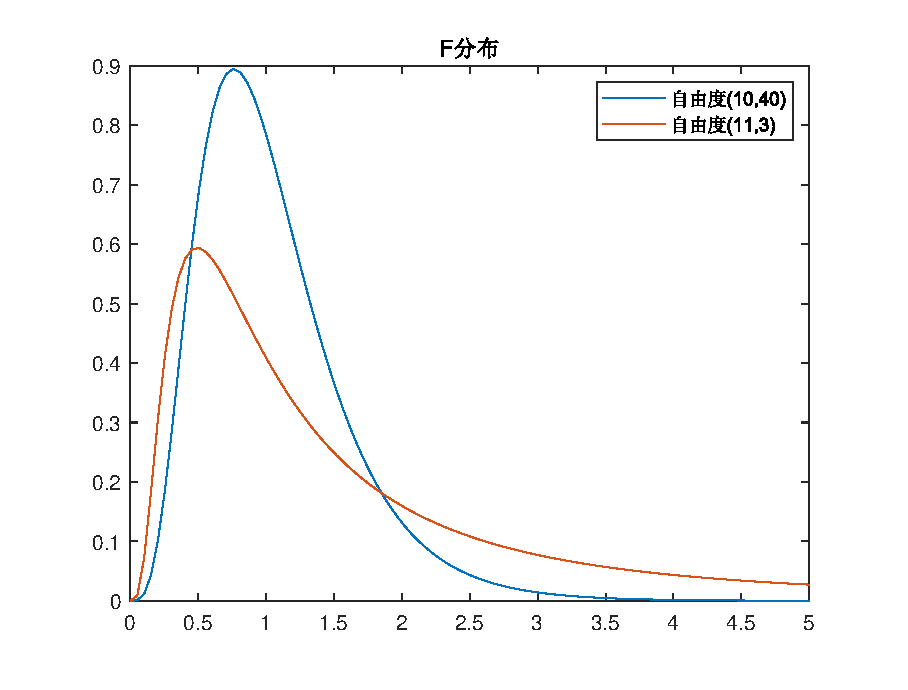
\includegraphics[width = 0.9\textwidth]{images/fdistribution.eps}
	\end{frame}


	\begin{frame}{抽样分布}
		例: 如果$X\sim \chi^2(n),Y\sim \chi^2(m)$,$X,Y$独立,则$X+Y\sim \chi^2(n+m)$
		
		证明: 取$X_1,X_2,\dots,X_{n+m}$独立同分布,都服从标准正态分布.此时有
		$(X,Y)$和$\big(\sum\limits_{i=1}^{n}X_i^2,\sum\limits_{j=n+1}^{n+m}X_i^2 \big)$同分布,于是
		$X+Y$和$\sum\limits_{i=1}^{n+m}X_i^2$同分布.即有$X+Y\sim \chi^2(n+m)$. 证毕.
		\\ \hspace*{\fill} \\
		例: 设$X_1,\dots,X_n$是来自总体$N(0,1)$的样本.
		\begin{equation}
			\overline{X} = \frac{1}{n}\sum_{j=1}^{n}X_j,\quad S^2 = \frac{1}{n-1}\sum_{j=1}^{n}(X_j-\overline{X})^2
		\end{equation}
		分别是样本均值和样本方差,则
		
		(1) $\overline{X}$和$S^2$独立 \\
		(2) $(n-1)S^2\sim \chi^2(n-1)$.
	\end{frame}
	
	\begin{frame}{抽样分布}
		证明: 引入正交矩阵
		\begin{equation}
			\bm{T} = \frac{1}{\sqrt{n}} 
			\begin{pmatrix} 
				1 & 1 & \dots & 1 \\
				* & * & \dots & * \\ 
				\vdots & \vdots & & \vdots \\
				* & * & \dots & * 
			 \end{pmatrix}.
		\end{equation}
		由$\bm{X}=(X_1,\dots,X_n)^{\mathrm{T}}\sim N(\bm{0},\bm{I})$知道$\bm{Y}=\bm{TX}\sim N(\bm{0},\bm{I}) $,于是$Y_1,\dots,Y_n$独立同分布且都服从于标准正态分布.利用$\overline{X}=Y_1/\sqrt{n}$和
		\begin{equation}
			\sum_{j=1}^{n}X_j^2 = \bm{X}^{\mathrm{T}}\bm{X} = \bm{Y}^{\mathrm{T}}\bm{Y} = 	\sum_{j=1}^{n}Y_j^2
		\end{equation}
	\end{frame}
	
	\begin{frame}{抽样分布}
		得到:
		\begin{equation}
			\begin{split}
				(n-1)S^2 &= \sum_{j=1}^{n}X_j^2 - n\overline{X}^2 \\
				&= \sum_{j=1}^{n}Y_j^2 - Y_1^2 \\
				&= \sum_{j=2}^{n}Y_j^2 \sim \chi^2(n-1)
			\end{split}
		\end{equation}
		并且和$\overline{X}=Y_1/\sqrt{n}$独立.
	\end{frame}

	\begin{frame}{抽样分布}
		\alert{
		练习: 如果$X_1,X_2,\dots,X_n$是总体$N(\mu,\sigma^2)$的样本,证明:
		
		(1) $\overline{X}$和$S^2$独立\\
		(2) $\frac{(n-1)S^2}{\sigma^2}\sim \chi^2(n-1)$.
		}
		证明:
		
		令
		\begin{equation}
			Y_j = \frac{X_j-\mu}{\sigma},
		\end{equation}
		则$Y_1,\dots,Y_n$独立同分布于标准正态分布.
		\begin{equation}
			\overline{X} = \mu + \sigma\overline{Y},\frac{(n-1)S^2}{\sigma^2} = \sum_{j=1}^{n}(Y_j-\overline{Y})^2
		\end{equation}
		由上题的结论知道$\overline{X}$和$S^2$独立,且$\sum_{j=1}^{n}(Y_j-\overline{Y})^2\sim \chi^2(n-1)$.
	\end{frame}

	\begin{frame}

		练习(非中心$\chi^2$分布):如果$X_1,X_2,\dots,X_n$相互独立,$X_i$服从$N(\mu_i,1)$,令$Z=X_1^2+X_2^2+\dots+X_n^2$.证明:
		
		(1) $Z$的概率密度函数为:
		\begin{equation}
		f_Z(z) = e^{-\theta/2}e^{-z/2}\sum_{j=0}^{+\infty}\frac{1}{j!}\frac{(\theta/2)^j}{2^{j+n/2}\Gamma(j+n/2)}z^{j+n/2-1},z>0;
		\end{equation}
		(2)$Z$的特征函数$\mathrm{E}e^{itZ} = \frac{1}{(1-2it)^{n/2}}\exp(\frac{it\theta}{1-2it})$,
		
		其中,$\theta = \mu_1^2+\dots+\mu_n^2>0$.
		\\ \hspace*{\fill} \\%空行
		Rmk:在统计中称$Z$服从自由度为$n$、非中心参数为$\delta = \sqrt{\theta}$的非中心$\chi^2$分布,记作$Z\sim \chi^2(n,\delta)$.
	\end{frame}

	\begin{frame}
		证明:
		
		(1)作正交矩阵
		\begin{equation}
		\bm{T} = \frac{1}{\sqrt{\theta}} 
		\begin{pmatrix} 
		\mu_1 & \mu_2 & \dots & \mu_n \\
		* & * & \dots & * \\ 
		\vdots & \vdots & & \vdots \\
		* & * & \dots & * 
		\end{pmatrix}.
		\end{equation}
		由于$\bm{X} = (X_1,\dots,X_n)^{\mathrm{T}}\sim N(\bm{\mu},\bm{I})$,其中$\bm{\mu}=(\mu_1,\dots,\mu_n)^{\mathrm{T}}$.
		
		令$\bm{Y} = (Y_1,\dots,Y_n) = \bm{TX}$,则$\bm{Y}\sim N(\bm{T\mu},\bm{I})$,因此,有$Y_1,\dots,Y_n$独立, $Y_i\sim N(b_i,1)$,按$\bm{T}$的取法,有:
		$b_1=\sqrt{\theta},b_2=\dots=b_n=0.$		
		
		记$W=\sum\limits_{j=2}^{n}Y_j^2$,则$Z=W+Y_1^2$,其中,$W$与$Y_1^2$独立,而$W\sim\chi^2(n-1),Y_1\sim N(\sqrt{\theta},1)$.
	\end{frame}

	\begin{frame}
		容易算出: $Y_1^2$有密度:
		\begin{equation}
			\begin{split}
				g(x) &= \frac{1}{2\sqrt{2\pi x}}\bigg[\exp(-\frac{(\sqrt{x}-\sqrt{\theta})^2}{2})+\exp(-\frac{(-\sqrt{x}-\sqrt{\theta})^2}{2})\bigg]\bm{1}_{(x>0)} \\
				&= \frac{1}{2\sqrt{2\pi x}} e^{-\theta/2}e^{-x/2}(e^{\sqrt{\theta x}}+e^{-\sqrt{\theta x}})\bm{1}_{(x>0)} \\
				&= \frac{1}{2\sqrt{2\pi }} e^{-\theta/2}e^{-x/2}\sum_{j=0}^{+\infty}\frac{1}{(2j)!}\theta^{j}x^{j-1/2}\bm{1}_{(x>0)}
			\end{split}
		\end{equation}
		
		回忆$W\sim\chi^2(n-1)$的密度函数:
		\begin{equation}
			k_{n-1}(x) = \frac{1}{2^{(n-1)/2}\Gamma(\frac{n-1}{2})}x^{(n-1)/2-1}e^{-x/2}\bm{1}_{(x>0)}
		\end{equation}
	\end{frame}

	\begin{frame}
		按和的密度公式,定出$Z$的概率密度函数为
		\begin{equation}
			\begin{split}
				f_Z(z) &= \int_{-\infty}^{\infty}g(u)k_{n-1}(z-u)\mathrm{d}u \\
				&= \int_{-\infty}^{\infty}\frac{1}{2\sqrt{2\pi }} e^{-\theta/2}e^{-u/2}\sum_{j=0}^{+\infty}\frac{1}{(2j)!}\theta^{j}u^{j-1/2}\bm{1}_{(u>0)} \\
				&\times\frac{1}{2^{(n-1)/2}\Gamma(\frac{n-1}{2})}(z-u)^{(n-1)/2-1}e^{-(z-u)/2}\bm{1}_{(z-u>0)}\mathrm{d}u \\
				&= \int_{0}^{z}\frac{1}{2\sqrt{2\pi }} e^{-\theta/2}e^{-u/2}\sum_{j=0}^{+\infty}\frac{1}{(2j)!}\theta^{j}u^{j-1/2}\\
				&\times\frac{1}{2^{(n-1)/2}\Gamma(\frac{n-1}{2})}(z-u)^{(n-1)/2-1}e^{-(z-u)/2}\mathrm{d}u \bm{1}_{(z>0)}
			\end{split}
		\end{equation}
	\end{frame}

	\begin{frame}
		将上式稍作整理得到:
		\begin{equation}
			\begin{split}
				f_Z(z) &= 
					\frac{1}{2\sqrt{2\pi}}e^{-\frac{\theta}{2}}\frac{1}{2^{\frac{n-1}{2}}\Gamma(\frac{n-1}{2})}\sum_{j=0}^{+\infty}\theta^je^{-z/2} \\
					&\times\int_{0}^{z}u^{j-1/2}(z-u)^{(n-1)/2-1}\mathrm{d}u \bm{1}_{(z>0)}.
			\end{split}
		\end{equation}
		利用Gamma函数和Beta函数的关系:
		\begin{equation}
			\begin{split}
					\int_{0}^{x}y^a(x-y)^b\mathrm{d}y &= x^{a+b+1}\int_{0}^{1}t^a(1-t)^b\mathrm{d}t \\
					&= x^{a+b+1}\mathrm{B}(a+1,b+1) \\
					&= x^{a+b+1}\frac{\Gamma(a+1)\Gamma(b+1)}{\Gamma(a+b+2)}.
			\end{split}
		\end{equation}
	\end{frame}

	\begin{frame}
		化简得到:
		\begin{equation}
			f_Z(z) =e^{-\theta/2}e^{-z/2}\sum_{j=0}^{+\infty}\frac{1}{j!}\frac{(\theta/2)^j}{2^{j+n/2}\Gamma(j+n/2)}z^{j+n/2-1}\bm{1}_{(z>0)}
		\end{equation}
		(2)要计算$Z$的特征函数$\mathrm{E}e^{itZ}$
		
		若用定义
		\begin{equation}
			\mathrm{E}e^{itZ} = \int_{-\infty}^{\infty}f_Z(z)e^{itz}dz
		\end{equation}
		$\longrightarrow$糟糕!
		\\ \hspace*{\fill} \\%空行
		注意到:$Z=X_1^2+X_2^2+\dots+X_n^2$,并且$X_1,X_2,\dots,X_n$相互独立,于是有:
		\begin{equation}
			\mathrm{E}e^{itZ} = \mathrm{E}e^{itX_1^2}\cdots\mathrm{E}e^{itX_n^2}.
		\end{equation}
	\end{frame}

	\begin{frame}
		注意到:$X_{k}^{2}$有特征函数
		\begin{equation}
			\mathrm{E}e^{itX_{k}^{2}}=\int_{-\infty }^{+\infty}{{{e}^{it{{x}^{2}}}}\frac{1}{\sqrt{2\pi }}{{e}^{-\frac{{{(x-{{\mu }_{k}})}^{2}}}{2}}}\mathrm{d}x}=\frac{1}{\sqrt{2\pi }}\int_{-\infty }^{+\infty }{{{e}^{M(x)}}\mathrm{d}x}
		\end{equation}
		
		其中$M(x)=it{{x}^{2}}-\frac{{{(x-{{\mu }_{k}})}^{2}}}{2}=-\frac{(1-2it)}{2}{{(x-\frac{{{\mu }_{k}}}{1-2it})}^{2}}+\frac{i\mu _{k}^{2}t}{1-2it}.$ 
		
		因此,
		\begin{equation}
			\begin{split}
					\mathrm{E}e^{itX_{k}^{2}} &=\frac{1}{\sqrt{2\pi }}\int_{-\infty }^{+\infty }{{{e}^{-\frac{(1-2it)}{2}{{(x-\frac{{{\mu }_{k}}}{1-2it})}^{2}}+\frac{i\mu _{k}^{2}t}{1-2it}}}dx} \\
					&=\frac{1}{\sqrt{2\pi }}{{e}^{\frac{i\mu _{k}^{2}t}{1-2it}}}\int_{-\infty }^{+\infty }{{{e}^{-\frac{(1-2it)}{2}{{y}^{2}}}}dy} \\
					&=\frac{1}{{{(1-2it)}^{1/2}}}\exp \left( \frac{it\mu _{k}^{2}}{1-2it} \right),
			\end{split}
		\end{equation}
		
	\end{frame}

	\begin{frame}
		最后,
		\begin{equation}
			\begin{split}
				\mathrm{E}e^{itZ} &= \mathrm{E}e^{itX_1^2}\cdots\mathrm{E}e^{itX_n^2} \\
				&= \frac{1}{{{(1-2it)}^{n/2}}}\exp \left( \frac{it\theta}{1-2it} \right).
			\end{split}
		\end{equation}
		练习(非中心$t$分布): 设$X\sim N(\delta,1),Y\sim \chi^2(n)$,求$T = \frac{X}{\sqrt{Y/n}}$的密度函数,其中$\delta\in\mathbb{R}$.
		Ans:
		\begin{equation}
			\begin{split}
				h_{n,\delta}(x) &= \frac{n^{n/2}}{\sqrt{\pi}\Gamma(\frac{n}{2})}e^{-\delta^2/2}(n+x^2)^{-(n+1)/2} \\
				&\times \sum_{j=0}^{\infty}\Gamma(\frac{n+j+1}{2})\frac{(\delta x)^j}{j!}(\frac{2}{n+x^2})^{j/2}.
			\end{split}
		\end{equation}
	\end{frame}

	\begin{frame}
		练习(非中心$F$分布):设$X,Y$独立,$X\sim\chi^2(n),Y\sim\chi^2(m,\delta)$,求$Z=\frac{Y/m}{X/n}$的密度函数.
		\\ \hspace*{\fill} \\%空行
		Ans:
		\begin{equation}
			\begin{split}
				f_{m,n,\delta}(x) &= e^{-\delta^2/2}\sum_{j=0}^{\infty}\frac{(\delta^2/2)^j}{j!}n^{n/2}m^{m/2+j} \\
				&\times \frac{\Gamma(\frac{1}{2}(m+n)+j)}{\Gamma(\frac{n}{2})\Gamma(\frac{m}{2}+j)}
				\frac{x^{m/2-1+j}}{(n+mx)^{(m+n)/2+j}}\bm{1}_{(x>0)}.
			\end{split}
		\end{equation}
	\end{frame}

	\begin{frame}
		练习: 设$X\sim\chi^2(2n),n$为正整数,设$a>0$,$Y\sim\mathcal{P}(\frac{a}{2})$(Poisson分布).
		
		证明:
		\begin{equation}
			P(X<a) = P(Y\geqslant n).
		\end{equation}
		证明: \begin{equation}
			P(X<a) = \frac{1}{2^n\Gamma(n)}\int_{0}^{a}x^{n-1}e^{-x/2}\mathrm{d}x
		\end{equation}
		反复利用分部积分公式:
		\begin{equation}
			\begin{split}
				P(X<a) &= \frac{1}{2^n(n-1)!}\int_{0}^{a}x^{n-1}e^{-x/2}\mathrm{d}x \\
				&= \frac{1}{2^n(n-1)!}\int_{x=0}^{a}e^{-x/2}\mathrm{d}\left(\frac{x^n}{n}\right) \\
				&= \frac{a^n}{2^nn!}e^{-a/2}+\frac{1}{2^{n+1}n!}\int_{0}^{a}x^{n}e^{-x/2}\mathrm{d}x \\
				&= \sum_{k=n}^{n+r}\frac{a^k}{2^kk!}e^{-a/2}+\frac{1}{2^{n+r+1}(n+r)!}\int_{0}^{a}x^{n+r}e^{-x/2}\mathrm{d}x.
			\end{split}
		\end{equation}
	\end{frame}

	\begin{frame}
		放缩:
		\begin{equation}
			\begin{split}
				0&<\frac{1}{2^{n+r+1}(n+r)!}\int_{0}^{a}x^{n+r}e^{-x/2}\mathrm{d}x \\ &<\frac{1}{2^{n+r+1}(n+r)!}\int_{0}^{a}x^{n+r}\mathrm{d}x \\
				&=\frac{1}{2^{n+r+1}(n+r)!}\frac{a^{n+r+1}}{n+r+1} \\
				&=\frac{(a/2)^{n+r+1}}{(n+r+1)!}\rightarrow 0(r\rightarrow\infty)
			\end{split}
		\end{equation}
		(回忆:数学分析中的"阶指幂对"原理.	)
		
		令$r\rightarrow\infty$即得结论
	\end{frame}

	\begin{frame}
		练习:把$\chi^2$分布推广到$n$非整数的情况:$Z$服从$\chi^2(a)$分布,则$Z$是有密度
		\begin{equation}
			f_Z(z)=\frac{1}{2^{a/2}\Gamma(a/2)}z^{a/2-1}e^{-z/2}\bm{1}_{(x>0)}
		\end{equation}
		的随机变量.
		证明: 
		\alert{
		\begin{equation}
			\mathrm{E}Z = a,\mathrm{var}Z=2a;
		\end{equation}
		}
		且当$a\rightarrow\infty$时,
		\begin{equation}
			\frac{Z-a}{\sqrt{2a}}\stackrel{d}{\longrightarrow}N(0,1).
		\end{equation}
	\end{frame}

	\begin{frame}
		证明:由$Z$的概率密度
		\begin{equation}
			f(z) = \frac{1}{2^{a/2}\Gamma(a/2)}z^{a/2-1}e^{-z/2},z>0
		\end{equation}
		得到:
		\begin{equation}
			\begin{split}
				\mathrm{E}(Z^k) &= \int_{-\infty }^{\infty}z^kf(z)\mathrm{d}z \\
				&= \int_{0}^{\infty}\frac{1}{2^{a/2}\Gamma(a/2)}z^{a/2+k-1}e^{-z/2}\mathrm{d}z \\
				&= \int_{0}^{\infty}\frac{2^k}{\Gamma(a/2)}t^{a/2+k-1}e^{-t}\mathrm{d}t \\
				&= \frac{2^k\Gamma(a/2+k)}{\Gamma(a/2)}
			\end{split}
		\end{equation}
		因此,$\mathrm{E}Z = a,\mathrm{E}Z^2 = 4(\frac{a}{2}+1)(\frac{a}{2}) =a(a+2),\mathrm{var}Z=2a. $
	\end{frame}

	\begin{frame}
		还注意到:$Z$有特征函数
		\begin{equation}
		\phi_Z(t) = \mathrm{E}e^{itZ} = \frac{1}{\left(1-2it\right)^{a/2}}
		\end{equation}
		因此,随机变量$\frac{Z-a}{\sqrt{2a}}$的特征函数为
		\begin{equation}
		\begin{split}
		\mathrm{E}e^{it\frac{Z-a}{\sqrt{2a}}}&=e^{-it\frac{a}{\sqrt{2a}}}\mathrm{E}e^{i\frac{t}{\sqrt{2a}}Z} = e^{-it\frac{a}{\sqrt{2a}}}\frac{1}{\left(1-2i\frac{t}{\sqrt{2a}}\right)^{a/2}} \\
		&= \exp\left(-it\frac{a}{\sqrt{2a}}-\frac{a}{2}\ln(1-2i\frac{t}{\sqrt{2a}})\right) \\
		&= \exp\left(-it\frac{a}{\sqrt{2a}}+it\frac{a}{\sqrt{2a}}-\frac{a}{2}\frac{1}{2}\frac{4t^2}{2a}+o(\frac{1}{\sqrt{a}})  \right)\\
		&=\exp\left(-\frac{1}{2}t^2+o(\frac{1}{\sqrt{a}})  \right)\rightarrow e^{-\frac{t^2}{2}}
		\end{split}
		\end{equation}证毕.
	\end{frame}

	\begin{frame}
		例: 如果$X_1,\dots,X_n$是总体$N(\mu,\sigma^2)$的样本,则:
		\alert{
			\begin{equation}
				\frac{\overline{X}-\mu}{S/\sqrt{n}}\sim t(n-1).
			\end{equation}
		}
		证明:
		\begin{equation}
			Z = \frac{\overline{X}-\mu}{\sigma/\sqrt{n}}\sim N(0,1),\xi = \frac{n-1}{\sigma^2}S^2\sim\chi^2(n-1).
		\end{equation}
		$Z$和$\xi$独立,于是:
		\begin{equation}
			\frac{\overline{X}-\mu}{S/\sqrt{n}} = \frac{Z}{\sqrt{\xi/(n-1)}}\sim t(n-1).
		\end{equation}
	\end{frame}

	\begin{frame}
		例:设$X_1,\dots,X_n$是来自总体$N(\mu_1,\sigma_1^2)$的样本,$Y_1,\dots,Y_n$是来自总体$N(\mu_2,\sigma_2^2)$的样本,又设这两个总体是相互独立的,则当$m,n\geqslant 2$时,
		\alert{
			\begin{equation}
				\frac{S_X^2/\sigma_1^2}{S_Y^2/\sigma_2^2}\sim F(n-1,m-1).
			\end{equation}
		}
		其中
		\begin{equation}
			S_X^2 = \frac{1}{n-1}\sum_{j=1}^{n}(X_j-\overline{X})^2,S_Y^2 = \frac{1}{m-1}\sum_{j=1}^{m}(Y_j-\overline{Y})^2
		\end{equation}
		证明:由于$(n-1)S_X^2/\sigma_1^2\sim\chi^2(n-1),(m-1)S_Y^2/\sigma_2^2\sim\chi^2(m-1)$且二者独立,
		
		由$F$分布的定义知结论成立.
	\end{frame}

	\begin{frame}
		例:设$X_1,\dots,X_n$是来自总体$X\sim N(\mu_1,\sigma_1^2)$的样本,$Y_1,\dots,Y_n$是来自总体$Y\sim N(\mu_2,\sigma_2^2)$的样本,又设这两个总体是相互独立的,$\{X_i\}$和$\{Y_j\}$的样本均值、样本方差分别为:
		$\overline{X},\overline{Y},S_X^2,S_Y^2$.定义
		\begin{equation}
			S_W^2 = \frac{(n-1)S_X^2+(m-1)S_Y^2}{n+m-2},
		\end{equation}
		则,
		\alert{
			\begin{equation}
				Z=\frac{(\overline{X}-\overline{Y})-(\mu_1-\mu_2)}{\sqrt{\sigma_1^2/n+\sigma_2^2/m}}\sim N(0,1).
			\end{equation}
		}
	
		如果还有条件$\sigma_1^2 = \sigma_2^2 = \sigma^2$,则
		\alert{
			\begin{equation}
				T=\frac{(\overline{X}-\overline{Y})-(\mu_1-\mu_2)}{S_W\sqrt{1/n+1/m}}\sim t(n+m-2).
			\end{equation}
		}
	\end{frame}

	\begin{frame}
		证明:	由于总体$X,Y$独立,所以$X_1,\dots,X_n$与$Y_1,\dots,Y_n$独立.
		根据概率论的知识知道:
		\begin{equation}
			\overline{X}\sim N(\mu_1,\sigma_1^2/n),\overline{Y}\sim N(\mu_2,\sigma_2^2/m)
		\end{equation}
		利用$\overline{X},\overline{Y}$独立得到:
		\begin{equation}
			\overline{X}-\overline{Y} \sim N(\mu_1-\mu_2,\sigma_1^2/n+\sigma_2^2/m)
		\end{equation}
		于是得到$Z\sim N(0,1)$.
		再证$T\sim t(n+m-2)$.利用
		\begin{equation}
			\xi_1 = \frac{(n-1)S_X^2}{\sigma^2}\sim \chi^2(n-1),\xi_2 = \frac{(m-1)S_Y^2}{\sigma^2}\sim \chi^2(m-1),
		\end{equation}
		及$\xi_1,\xi_2$独立,得到:$\xi_1+\xi_2 \sim\chi^2(n+m-2)$.
	\end{frame}

	\begin{frame}
		简单计算,有:
		\begin{equation}
			S_W^2 = \frac{(\xi_1+\xi_2)\sigma^2}{n+m-2}
		\end{equation}
		又由于$Z,\xi_1,\xi_2$相互独立,于是$Z$与$\xi_1+\xi_2$独立.因此,
		\begin{equation}
			T=\frac{(\overline{X}-\overline{Y})-(\mu_1-\mu_2)}{S_W\sqrt{1/n+1/m}} = \frac{Z}{\sqrt{(\xi_1+\xi_2)/(n+m-2)}}\sim t(n+m-2).
		\end{equation}
		证毕.
	\end{frame}

	\begin{frame}
		例: 设$T$服从自由度是$n$的$t$分布,证明:
		若整数$k<n$,则$\mathrm{E}T^k$存在,若$k\geqslant n$,则$\mathrm{E}T^k$不存在.
		
		证明:
		
		研究积分\begin{equation}
			\begin{split}
				I_k &= \int_{-\infty}^{\infty} |t|^kf_T(t)\mathrm{d}t \\
				&= \int_{-\infty}^{\infty} a_n|t|^k\left(1+\frac{t^2}{n}\right)^{-(n+1)/2}\mathrm{d}t
			\end{split}
		\end{equation}
		由于$|t|^k\left(1+\frac{t^2}{n}\right)^{-(n+1)/2}\sim (\frac{1}{n})^{-(n+1)/2}|t|^{-(n+1)+k},(t\rightarrow\infty)$
		根据广义积分的比较审敛法知道:当且仅当$-(n+1)+k<-1$时,上式收敛,由此便得结论.
	\end{frame}

	\begin{frame}
		例:设$T$服从自由度是$n$的$t$分布,计算: \\
		(1)$\mathrm{E}T,(n\geqslant 2)$;\\
		(2)$\mathrm{var}T,(n\geqslant 3)$.
		
		解:(1)由$f_T(t)$关于$t=0$对称得到\alert{$\mathrm{E}T = 0,(n\geqslant 2)$};
		
		(2) 由于$\mathrm{E}T = 0$,所以$\mathrm{var}T = \mathrm{E}T^2$.
		
		将$T$表示成$T=\frac{X}{\sqrt{Y/n}}$,其中$X\sim N(0,1),Y\sim\chi^2(n)$,($X,Y$独立)就有:
		\begin{equation}
			\mathrm{E}T^2 = n\mathrm{E}X^2\mathrm{E}Y^{-1} = n\mathrm{E}Y^{-1}.
		\end{equation}
		前面曾经计算过:
		\begin{equation}
			\mathrm{E}Y^k = \frac{2^k\Gamma(a/2+k)}{\Gamma(a/2)}
		\end{equation}
		取$k=-1$得到:
		\begin{equation}
			\mathrm{E}Y^{-1} = \frac{2^{-1}\Gamma(n/2-1)}{\Gamma(n/2)} = (n-2)^{-1}.
		\end{equation}
		因此,\alert{$\mathrm{var}T = \frac{n}{n-2},(n\geqslant 3)$.}
	\end{frame}

	\begin{frame}
		例: (1)如果$X\sim F(n,m)$,则$X^{-1}\sim F(m,n)$
		
		(2)对$F(n,m)$分布的上$\alpha$分位数$F_{\alpha}(n,m)$,有:
		\alert{
		\begin{equation}
			F_{\alpha}(n,m) = \frac{1}{F_{1-\alpha}(m,n)}
		\end{equation}	
		}
		证明留作习题.
		
		(3)如果$X\sim F_{n,m}$,当$m>2$时,$\mathrm{E}X = \frac{m}{m-2}$.(仅与第二自由度有关)
		
		证明:表示$X = \frac{\xi_1/n}{\xi_2/m},$其中$\xi_1\sim\chi^2(n),\xi_2\sim\chi^2(m)$相互独立,
		\begin{equation}
			\mathrm{E}X = \frac{m}{n}\mathrm{E}\xi_1\mathrm{E}\frac{1}{\xi_2} = \frac{m}{n}n\mathrm{E}\frac{1}{m -_2} = \frac{m}{m-2}
		\end{equation}
	\end{frame}
